\chapter{Distributed Delay Model}

A systematic study of distributed delay in the context of Turing instabilities is extremely sparse in current literature, with no work having been previously done looking at the Schnakenberg model. In this chapter, we consider the LI model with time delay modelled as a symmetric truncated Guassian distribution. The quadrature rule we use to produce numerical simulations is first considered. The linear analysis conducted for the fixed delay case is then extended to the distributed delay model, and we look to show analytically that a symmetric truncated Gaussian distribution does not have a qualitative difference on the results seen, and thus does not resolve some of the key problems highlighted in the fixed delay case. These results are also verified through numerical simulations.

\section{Quadrature}\label{section:quad}

The LI model with distributed time delay, as defined in \eqref{distmodel}, is given as

\begin{equation}\label{distmodel2}
  \begin{split}
    \frac{\partial u}{\partial t}&=\frac{\epsilon^2}{L^2}\frac{\partial^2u}{\partial x^2}+a-u-2u^2v+3\int_{a}^{b}k(s,\tau,\sigma)\hat{u}^2\hat{v} \quad\text{ds},\\
    \frac{\partial v}{\partial t}&=\frac{1}{L^2}\frac{\partial^2v}{\partial x^2}+b-u^2v,
\end{split}
\end{equation}
where $\hat{u}=u(x,t-s)$ and $\hat{v}=v(x,t-s)$ where $s$ is the integration variable ranging over the delays. The function $k(s,\tau,\sigma)$ is the truncated Gaussian pdf for some mean $\tau$ and standard devation $\sigma$, and $\Phi_c$ is the truncation scaling constant. The integration domain $[a, b]$, with $a=\tau-n\sigma$ and $b=\tau+n\sigma$, can be discretised into $N$ sub-intervals of equal length with $N+1$ discretisation points, $s_0,\cdots,s_{N}$, such that $s_0=\tau-n\sigma$ and $s_N=\tau+n\sigma$. Using the composite Simpsons's rule \cite{compsimp}, the integral term can be numerically approximated as

\begin{equation}\label{simp}\int_{a}^{b}k(s)\hat{u}^2\hat{v}\  \text{ds}\approx\frac{h}{3}\left[k(s_0)\hat{u}^2_0\hat{v}_0+2\sum_{i=1}^{\frac{N}{2}-1}k(s_{2i})\hat{u}^2_{2i}\hat{v}_{2i}+4\sum_{i=2}^{\frac{N}{2}}k(s_{2i-1})\hat{u}^2_{2i-1}\hat{v}_{2i-1}+k(s_N)\hat{u}^2_N\hat{v}_N\right],
\end{equation}
where $h$ is computed as $h=\frac{b-a}{N}$. We use the notation $\hat{u}_j$ and $\hat{v}_j$ to denote $u(t-s_j)$ and $v(t-s_j$) respectively, namely the functions $u$ and $v$ evaluated at time-delay with some index $j$, $s_j$. Throughout the report we use $n=3$, so that the integration limits are $a=\tau-3\sigma$ and $b=\tau+3\sigma$. This was chosen so that a relatively large $\sigma$ value could be chosen for each $\tau$ while maintaining $a>0$.
Figures \ref{fig:pdf1} and \ref{fig:pdf2} show the pdf of a truncated Gaussian distribution centred at a mean $\tau=1,2$ with varying $\sigma$ values as fractions of $\sigma_{max}$. We have $s$ as the integration variable, with $s\in[a,b]$.

\begin{figure}[H]
    \centering
    \begin{subfigure}[b]{0.45\textwidth}
        \centering
        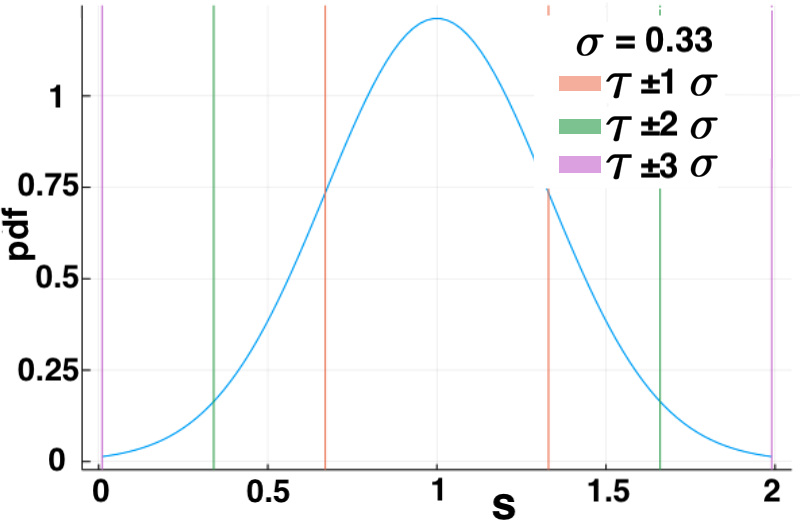
\includegraphics[width=7cm,height=5cm]{t1sig1.png}
        \caption{Truncated Gaussian distribution following $\mathcal{N}(1,(\sigma_{max}\times0.99)^2)$}
        \label{}
    \end{subfigure}
    \hfill
    \begin{subfigure}[b]{0.45\textwidth}
        \centering
        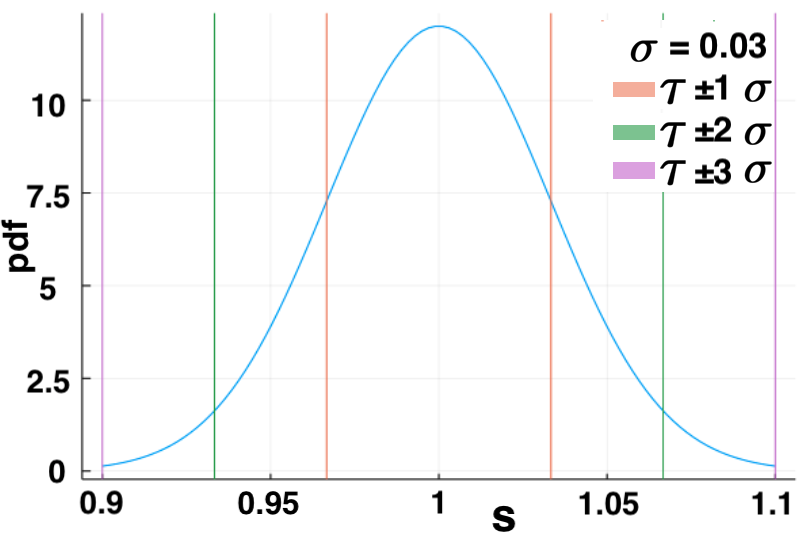
\includegraphics[width=7cm,height=5cm]{t1sig2.png}
        \caption{Truncated Gaussian distribution following $\mathcal{N}(1,(\sigma_{max}\times0.1)^2)$}
        \label{}
    \end{subfigure}
\caption{PDF of truncated Gaussian distribution with mean $\tau=1$ and integration domain $[1-3\sigma,1+3\sigma]$. $\sigma$ values of $0.33(2.d.p)$ and $0.03(2.d.p)$ are considered.}
\label{fig:pdf1}
\end{figure}
\begin{figure}[H]
    \centering
    \begin{subfigure}[b]{0.45\textwidth}
        \centering
        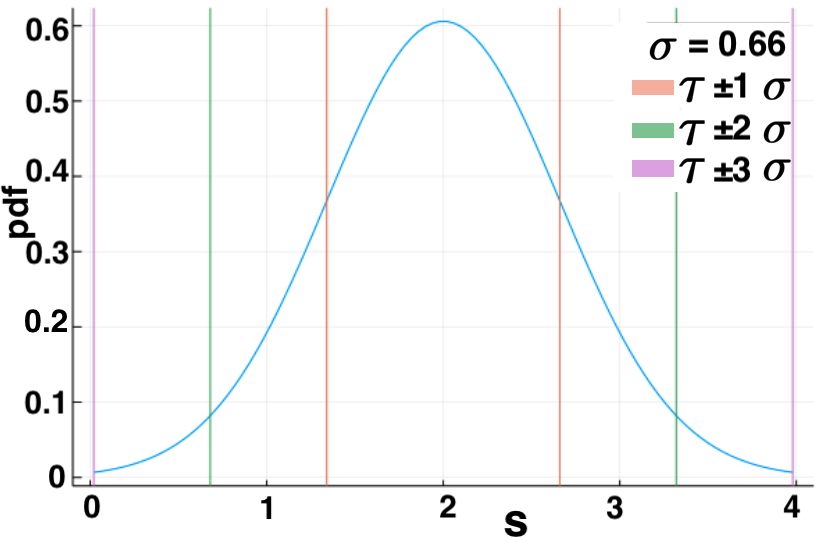
\includegraphics[width=7cm,height=5cm]{t2sig1.png}
        \caption{Truncated Gaussian distribution following $\mathcal{N}(2,(\sigma_{max}\times0.99)^2)$}
        \label{}
    \end{subfigure}
    \hfill
    \begin{subfigure}[b]{0.45\textwidth}
        \centering
        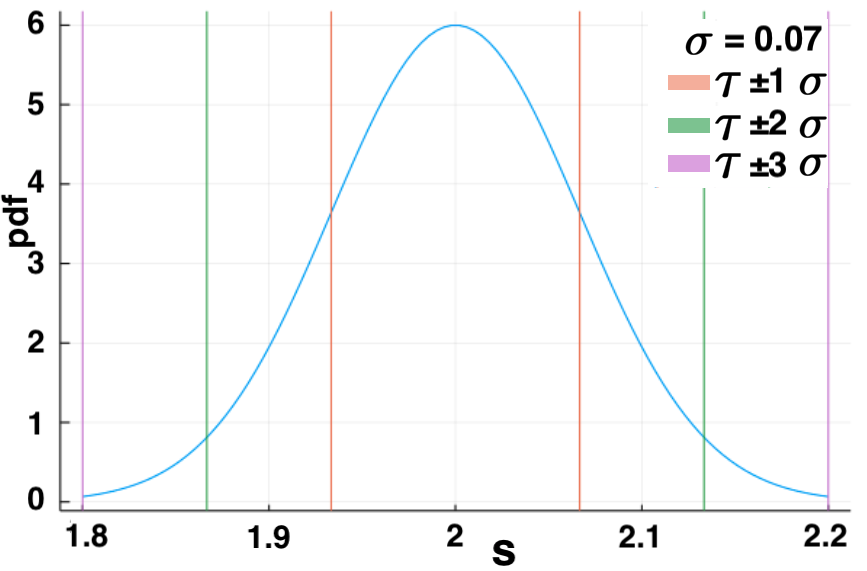
\includegraphics[width=7cm,height=5cm]{t2sig2.png}
        \caption{Truncated Gaussian distribution following $\mathcal{N}(2,(\sigma_{max}\times0.1)^2)$}
        \label{}
    \end{subfigure}
    \caption{PDF of truncated Gaussian distribution with mean $\tau=2$ and integration domain $[2-3\sigma,2+3\sigma]$. $\sigma$ values of $0.66(2.d.p)$ and $0.07(2.d.p)$ are considered.}
    \label{fig:pdf2}
\end{figure}
We see that $\sigma$ is responsible for scaling on the $x$-axis, while the truncation constant $\Phi_c$ scales the $y$-axis, ensuring the pdf integrates to $1$ across the integration domain. For the implementation of the quadrature rule, the number of sub-intervals $N$ was chosen to be $N=50$. The consideration for such a choice involves both quadrature accuracy and computational efficiency. The motivation for setting $N=50$ was dependant on evaluating `test' integrals and simulation `test' DDEs, for which the results are presented in the remainder of this section.

\section{Linear Analysis}\label{section:distlin}
Taking a small perturbation about the steady-state $u=u_\star+\delta\xi$, $v=v_\star+\delta\eta$, where $|\delta|\ll1$, we can write the equation for the activator $u$ in \eqref{distmodel2} as

\begin{equation}\label{perturb}
  \delta\frac{\partial \xi}{\partial t}=\delta \frac{\epsilon^2}{L^2}\frac{\partial^2\xi}{\partial x^2}+f(u_\star+\delta\xi, v_\star+\delta\eta)+g(u_\star+\delta\hat{\xi},v_\star+\delta\hat{\eta}) ,
\end{equation}
where $f(u,v)=a-u+2u^2v$ and $g(\hat{u},\hat{v})=3\int_a^bk(s)\hat{u}^2\hat{v} \text{ds}$. The $\hat{\xi}$ notation is used to denote the perturbation evaluated at a delay $\hat{\xi}=\xi(x,t-s)$. Taylor expanding equation \eqref{perturb} for the $f$ term about the steady-state and evaluating the $g$ term, up to $O(\epsilon)$, yields

\begin{dmath}\label{taylor}
  \delta\frac{\partial \xi}{\partial t}=\delta \frac{\epsilon^2}{L^2}\frac{\partial^2\xi}{\partial x^2}+f(u_\star,v_\star)+3u_\star^2v_\star\int_a^bk(s)\text{ds}+\delta\left[\xi f_u(u_\star,v_\star)+\eta f_v(u_\star,v_\star)+6u_\star v_\star\int_a^bk(s)\hat{\xi}\text{ds}+3u_\star^2\int_a^bk(s)\hat{\eta}\text{ds}
  \right].
\end{dmath}
We use the notation $f_u$ to denote the derivative of function $f$ with respect $u$. Using the facts that the truncated Guassian $k(s)$ integrates to $1$ over $[a,b]$, and evaluation the expressions $f_u(u_\star,v_\star)$ and $f_v(u_\star,v_\star)$, equation \eqref{taylor} can be simplified to

\begin{equation}\label{linu}
  \delta \frac{\partial \xi}{\partial t}=\delta \frac{\epsilon^2}{L^2}\frac{\partial^2\xi}{\partial x^2}+\delta\left[\xi(-1-4u_\star v_\star)-2\eta u_\star^2 +6u_\star v_\star\int_a^bk(s)\hat{\xi}\text{ds}+3u_\star^2\int_a^bk(s)\hat{\eta}\text{ds}\right].
\end{equation}
The linearised dynmacs for $v$ are more simply given by
\begin{equation}\label{linv}
\delta \frac{\partial\eta}{\partial t}=\delta \frac{1}{L^2}\frac{\partial^2\eta}{\partial x^2}-\delta\left[2\xi u_\star v_\star+\eta u_\star^2\right].
\end{equation}
Dividing through by $\delta$ and substituting in an ansatz of the form $\xi=\xi_0e^{\lambda t}\cos(k\pi x)$ \cite{yigaffneyli} into \eqref{linu} and $\eta=\eta_0e^{\lambda t}\cos(k\pi x)$ into \eqref{linv}, and then dividing through by $e^{\lambda t}$ and $\cos(k\pi x)$, results in

\begin{equation}\label{sysof}
  \begin{split}
\lambda\xi_0&=-\frac{\epsilon^2}{L^2}k^2\pi^2\xi_0+\xi_0(-1-4u_\star v_\star)-2\eta_0u_\star^2+6\xi_0u_\star v_\star E+3\xi_0u_\star^2E \\
\lambda\eta_0&=-\frac{1}{L^2}k^2\pi^2\eta_0-2\xi_0u_\star v_\star-\eta_0u_\star^2,
\end{split}
\end{equation}
where $E=\int_a^bk(s)e^{-\lambda s}\text{ds}$. We can write equation \eqref{sysof} as a homogeneous linear system for $(\xi_0,\eta_0)^T$, given by

\begin{equation}
\underbrace{\begin{pmatrix}-1-4u_\star v_\star-\frac{\epsilon^2}{L^2}k^2\pi^2+6u_\star v_\star E-\lambda&-2u_\star^2+3u_\star^2E\\-2u_\star v_\star&-u_\star^2-\frac{1}{L^2}k^2\pi^2-\lambda \end{pmatrix}}_{\textbf{M}}\begin{pmatrix}\xi_0\\\eta_0\end{pmatrix}=\begin{pmatrix}0\\0\end{pmatrix}.
\end{equation}
Looking for non-trivial solutions, we look for roots of the characteristic equation, namely $D_k=\text{det}(\textbf{M})=0$. The characteristic equation, $D_k$, is given as
\begin{equation}\label{characdist}
  D_k=\lambda^2+\alpha_k\lambda+\beta_k+(\gamma_k\lambda+\delta_k)E=0,
\end{equation}
where
\begin{align}
\alpha_k&=\left(\frac{\epsilon^2}{L^2}+\frac{1}{L^2}\right)k^2\pi^2+u_\star^2+4u_\star v_\star+1\\
\beta_k&=\left(\frac{1}{L^2}\pi^2k^2+u_\star^2\right)\left(\frac{\epsilon^2}{L^2}\pi^2k^2+4u_\star v_\star+1\right)-4u_\star^3v_\star\\
\gamma_k&=-6u_\star v_\star\\
\delta_k&=-\frac{6}{L^2}u_\star v_\star k^2\pi^2.
\end{align}

Finally, we note that the expression $E$ can be evaluated as
\begin{equation}
E=\int_a^bk(s)e^{-\lambda s}ds=\frac{\Phi_c}{2}\left[\exp\left(\frac{\lambda(\lambda\sigma^2-2\tau)}{2}\right) \text{erf} \left(\frac{\lambda\sigma^2+s-\tau}{\sqrt{2}\sigma}\right)\right]\Bigg|_a^b.
\end{equation}
The charactersitic equation \eqref{characdist} cannot trivially be split into it's real and imaginary components due to the error function term in $E$ as was done in the fixed delay case. We therefore cannot explicitly compute the stability lines in $(a,b)$ parameter space. We can however range over $(a,b)$ and compute $\max_k(\Re(\lambda_k))$ for different $\tau$, and produce plots similar to those in figures \ref{fig:dispfixed} and \ref{fig:lambdavary}. We use these plots to pseudo-analytically prove that, using a symmetric Gaussian distribution centred at mean $\tau$ will not change the time-to-pattern seen for a fixed delay of $\tau$, independent of the standard deviation of the distribution $\sigma$. We first plot $\max_k(\Re(\lambda_k))$ against $\tau$, as seen analogously in figure \ref{fig:dispfixed} for the fixed delay case, for multiple parameters $(a,b,\tau,\sigma)$, and compares these to the fixed delay case. Since physically we cannot have negative delays, we require the lower integration limit to be positive. Namely, for a given mean $\tau$, we require $\tau-3\sigma>0$. We therefore define a maximum $\sigma$ value by $\sigma_{max}=\tau / 3$. By ensuring $\sigma<\sigma_{max}$, we ensure only positive delays are considered.
\\\\
Figures \ref{fig:p1} and \ref{fig:p2} show $\max_k(\Re(\lambda_k))$ plotted against $\tau\in[0,1]$ for two different parameter sets $(a,b)=\{(0.1,0.9), (0.4,0.4)\}$, for the fixed delay case. For each parameter set, figures are produced with different $\sigma$ values as a fraction of $\sigma_{max}$, and the absolute value of the difference between $\max_k(\Re(\lambda))$ for each distributed delay case compared with the fixed delay case is plotted. We note that in the distributed delay case, as we vary $\tau$, $\sigma_{max}$ and thus the integration limits both change as functions of $\tau$. All numerical results in this chapter are produced with $L=30\sqrt{0.05}$, and unless otherwise stated, $\epsilon^2=0.001$.

% PARAMTER SET 2
\begin{figure}[H]
    \centering
    \begin{subfigure}[b]{0.45\textwidth}
        \centering
        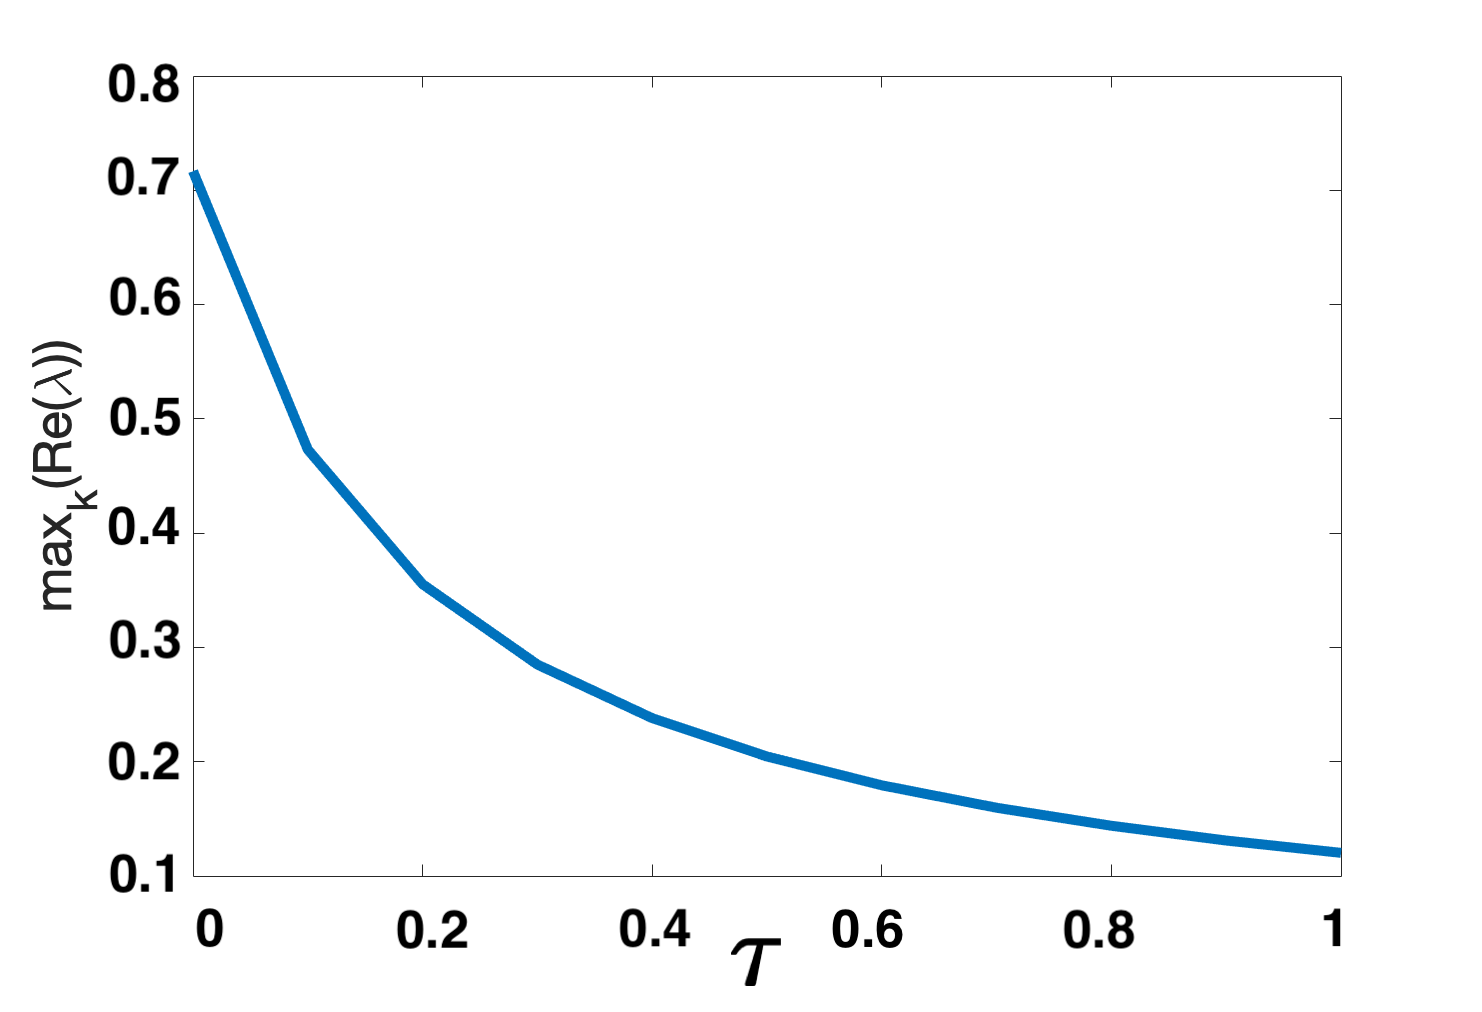
\includegraphics[width=7cm,height=5cm]{p2fixed.png}
        \caption{Fixed delay case.}
        \label{}
    \end{subfigure}
    \hfill
    \begin{subfigure}[b]{0.45\textwidth}
        \centering
        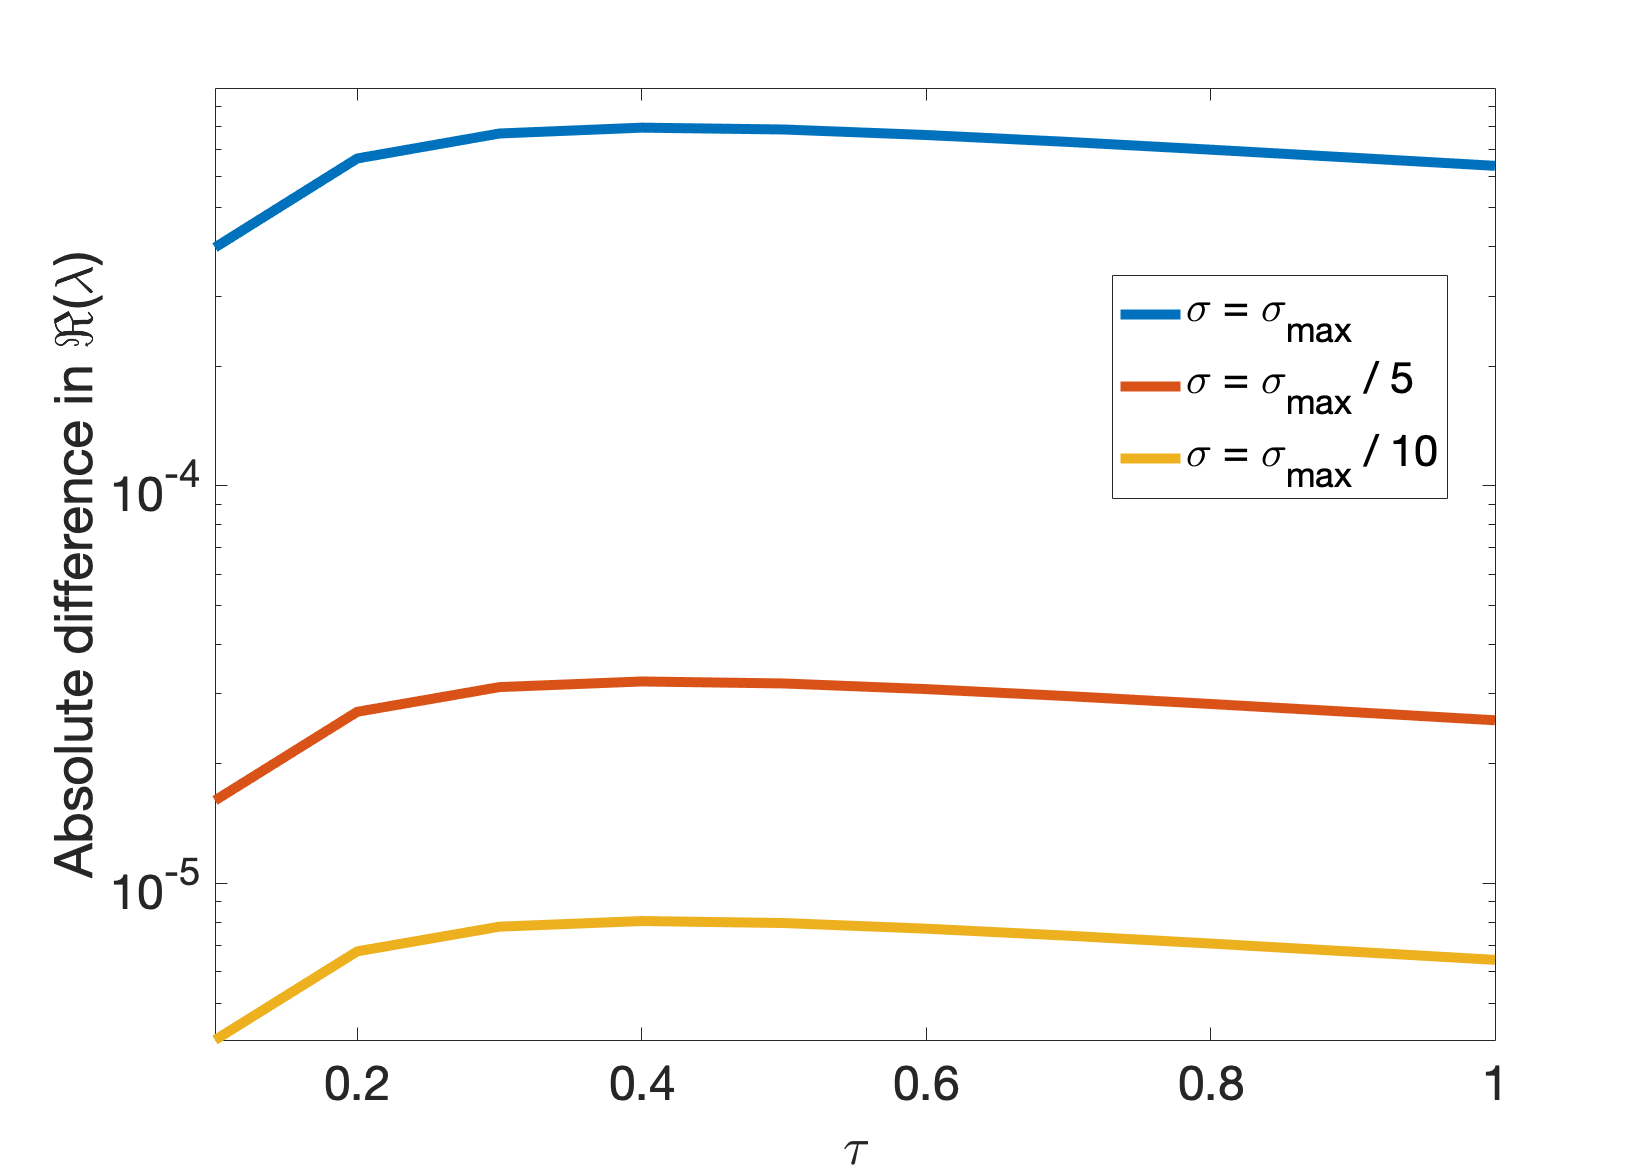
\includegraphics[width=7cm,height=5cm]{dispdiff1.png}
        \caption{Absolute difference in $\max_k(\Re(\lambda))$ as $\sigma$ is varied.}
        \label{}
    \end{subfigure}
    \caption{$\max_k(\Re(\lambda_k))$ plotted against $\tau\in[0,1]$ for parameter set $(a,b)=(0.1,0.9)$. $\epsilon^2=0.001$ and $L=30\sqrt{0.05}$. $k$ is varied over $[0,50]$ at regular discrete intervals of $1$.}
    \label{fig:p2}
\end{figure}
% PARAMETER SET 3
\begin{figure}[H]
    \centering
    \begin{subfigure}[b]{0.45\textwidth}
        \centering
        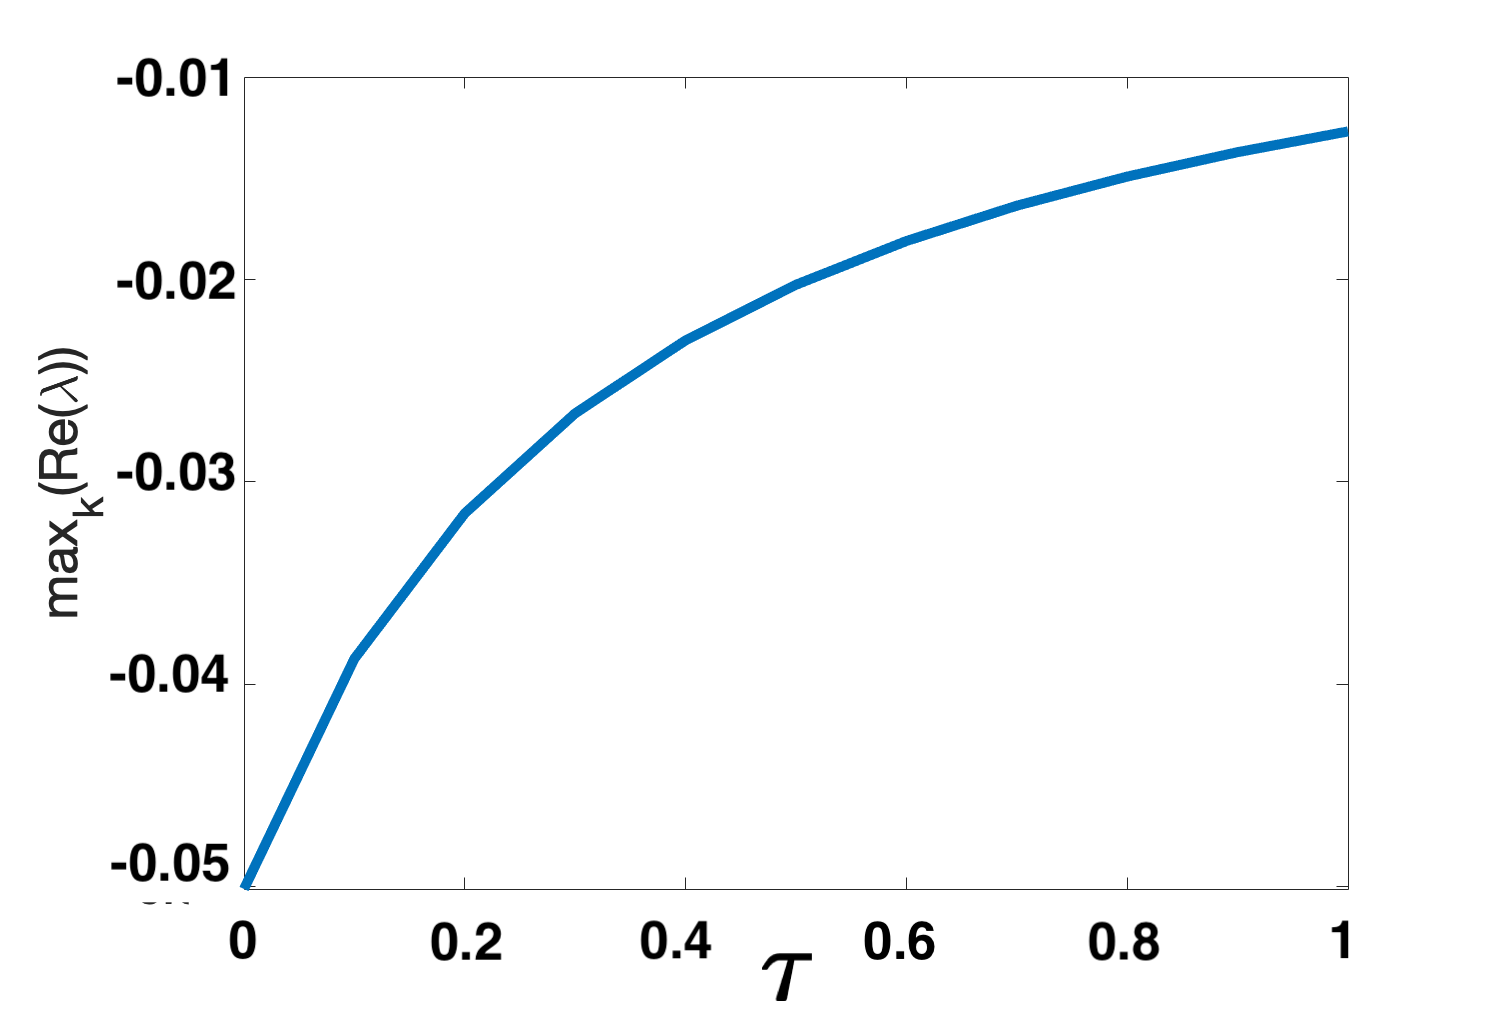
\includegraphics[width=7cm,height=5cm]{p3fixed.png}
        \caption{Fixed delay case.}
        \label{}
    \end{subfigure}
    \hfill
    \begin{subfigure}[b]{0.45\textwidth}
        \centering
        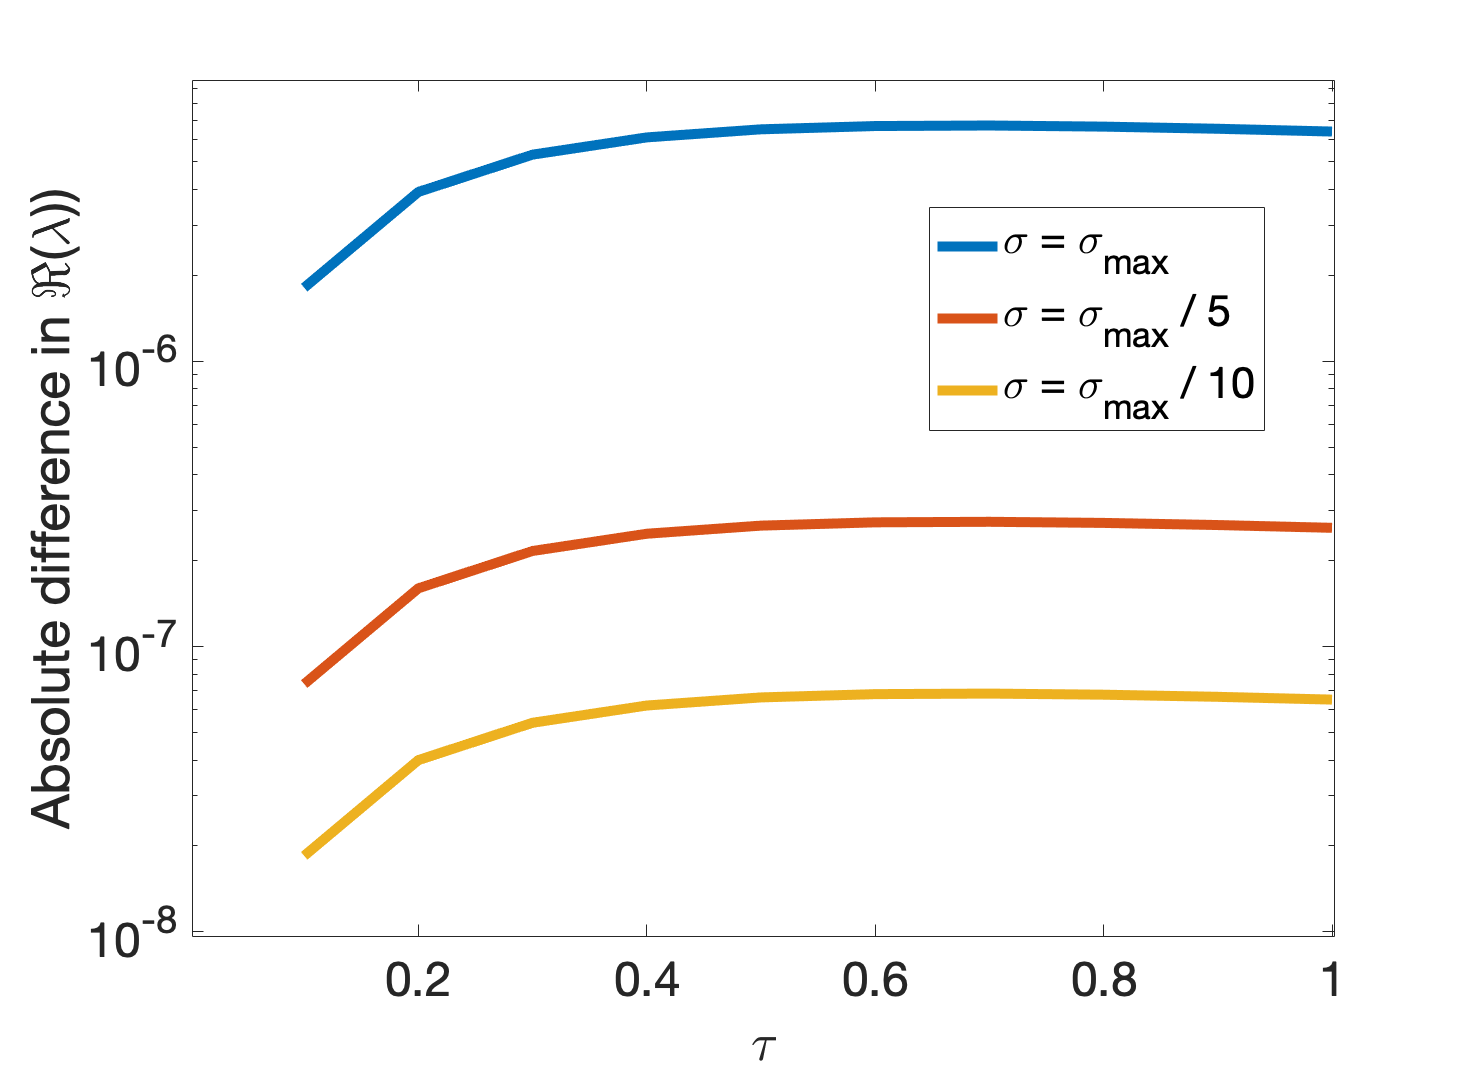
\includegraphics[width=7cm,height=5cm]{dispdiff2.png}
        \caption{Absolute difference in $\max_k(\Re(\lambda))$ as $\sigma$ is varied.}
        \label{}
    \end{subfigure}
    \caption{$\max_k(\Re(\lambda_k))$ plotted against $\tau\in[0,1]$ for parameter set $(a,b)=(0.4,0.4)$. $\epsilon^2=0.001$ and $L=30\sqrt{0.05}$. $k$ is varied over $[0,50]$ at regular discrete intervals of $1$.}
    \label{fig:p3}
\end{figure}

Figures \ref{fig:p2} and \ref{fig:p3} show that, the largest variation in $\max_k(\Re(\lambda))$ when the largest $\sigma$ value is used. The results also suggest that for all $\sigma$ and $\tau\in[0,1]$ considered, that we expect to see pattern formation for $(a,b)=(0.1,0.9)$, but not for $(a,b)=(0.4,0.4)$. We note that that largest absolute difference in $\max_k(\Re(\lambda))$ across both parameter sets is of $O(10^{-5})$. This is an extremely small difference, on a similar order to numerical round off error, and is thus unlikely to make a qualitative difference on time-to-pattern. We verify these obvservations numerically in section \ref{section:distsim}.
\\\\
 In order to consider how $max_k(\Re(\lambda))$ varies across a larger parameter plane as $\sigma$ is varied, we plot heatmaps of the absolute difference of $\max_k(\Re(\lambda_k))$ for varying $\sigma$ values as a fraction of $\sigma_{max}$, for $\tau\in\{0.2,1\}$, against the fixed delay case. Overlayed onto these bifurcation plots are the contour lines at $\max_k(\Re(\lambda_k))=0$ and $\Re(\lambda_0)=0$, to highlight the Turing instability region. For each $\tau$ and $\sigma$, the bifrucation plots were computed with two different $\epsilon^2$ values, $\epsilon^2=0.001,0.1$. Figures \ref{fig:distbif1} and \ref{fig:distbif3} show the results for a fixed $\tau=0.2$ with varying $\sigma$, and an $\epsilon^2=0.001,0.1$. Figures \ref{fig:distbif2} and \ref{fig:distbif4} show the analogous plots but with a fixed $\tau=1$.

\begin{figure}[H]
    \centering
    \begin{subfigure}[b]{0.45\textwidth}
        \centering
        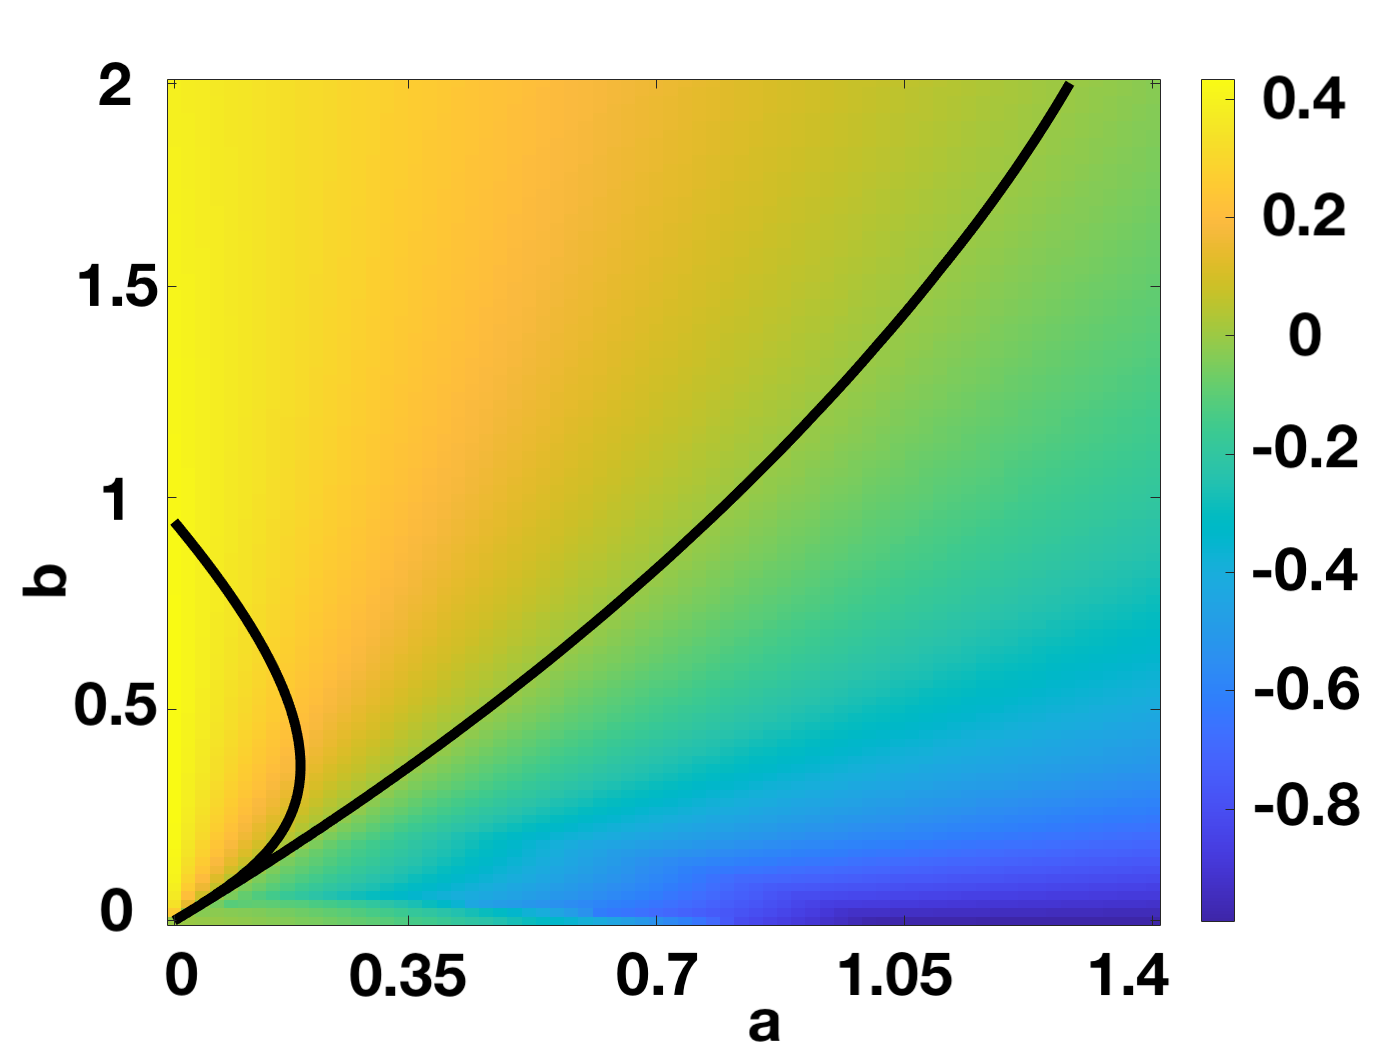
\includegraphics[width=7cm,height=4.75cm]{t1f1.png}
        \caption{Fixed delay case.}
        \label{}
    \end{subfigure}
    \hfill
    \begin{subfigure}[b]{0.45\textwidth}
        \centering
        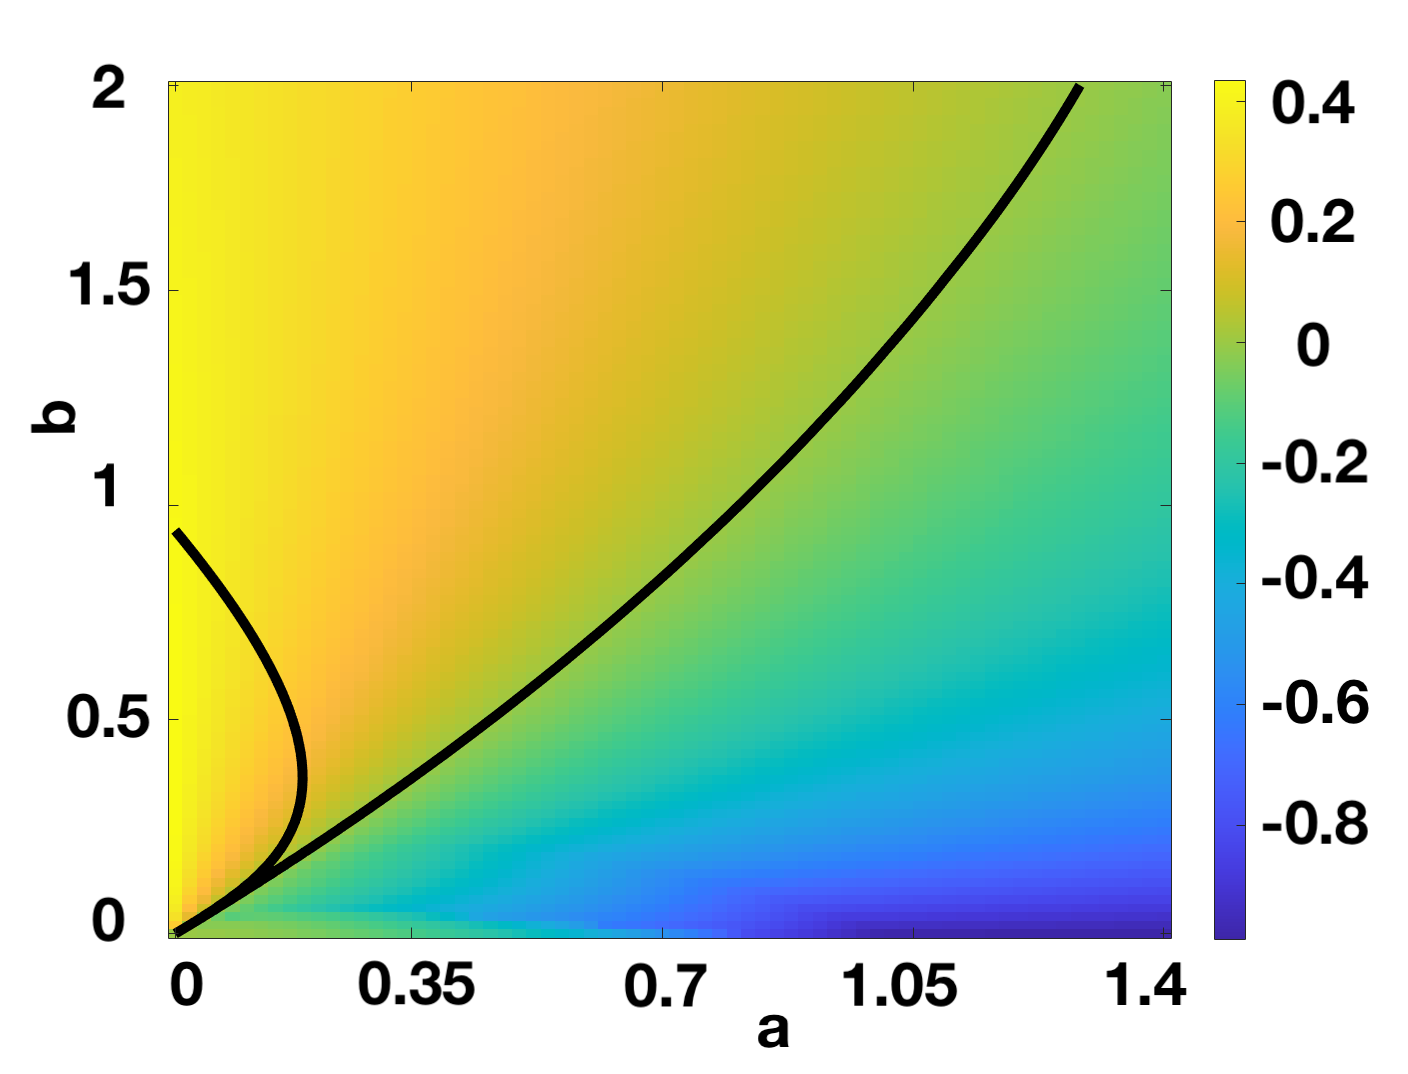
\includegraphics[width=7cm,height=4.75cm]{t1f2.png}
        \caption{Distributed delay with $\sigma=\sigma_{max}\times0.99$.}
        \label{}
    \end{subfigure}
    \hfill
    \begin{subfigure}[b]{0.45\textwidth}
        \centering
        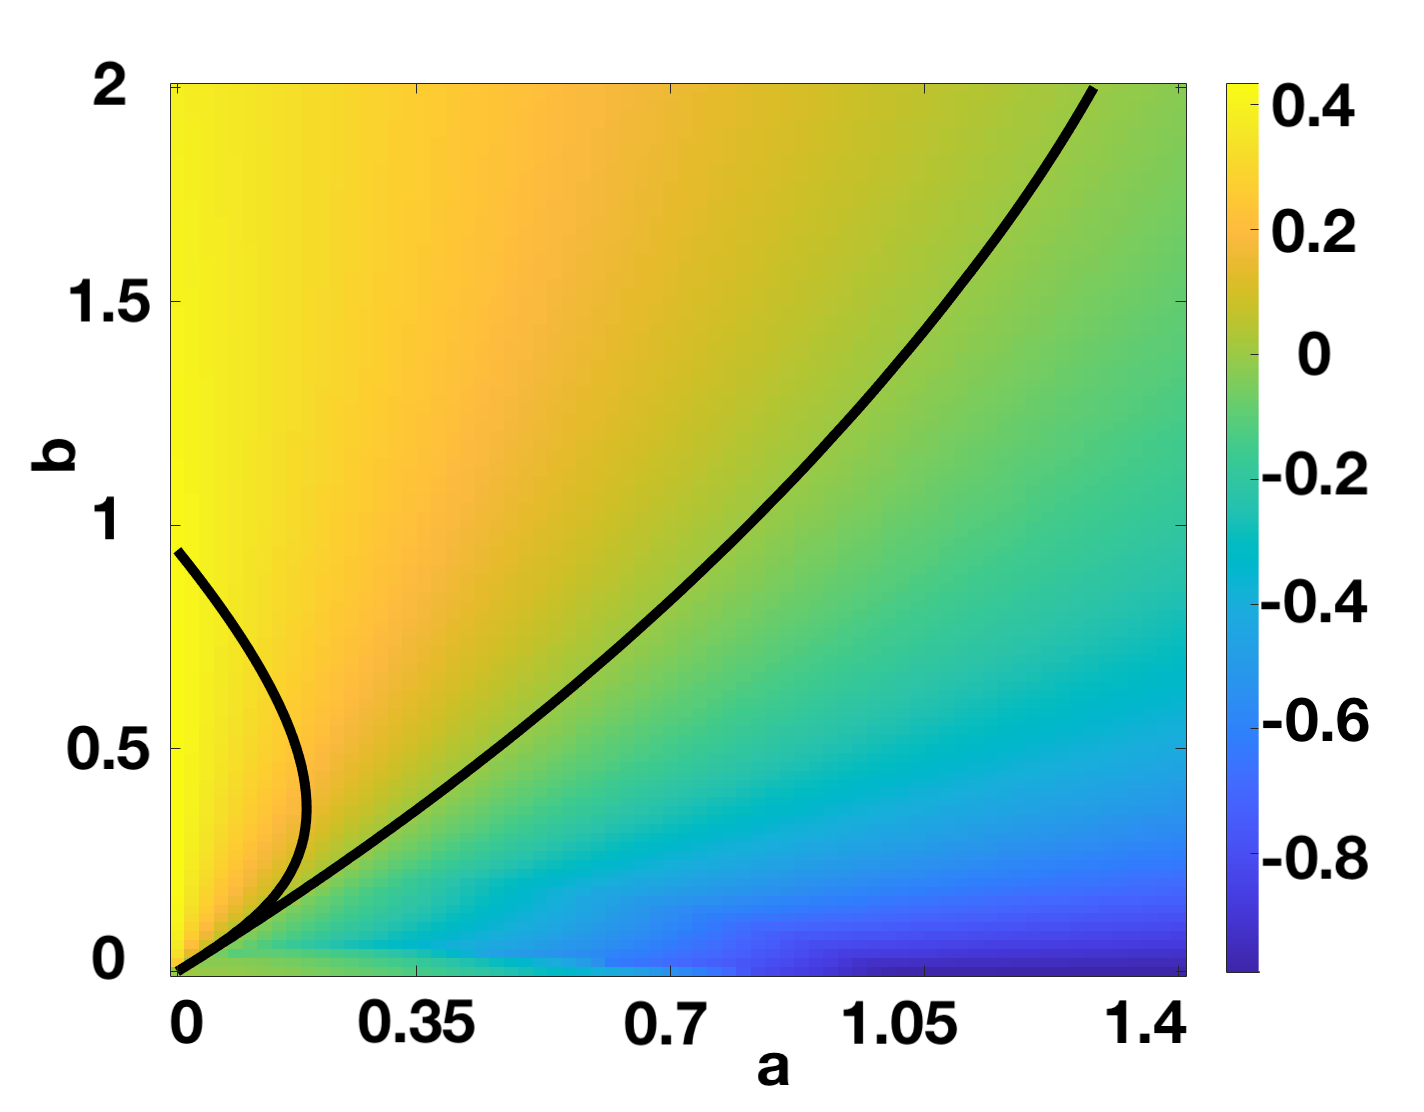
\includegraphics[width=7cm,height=4.75cm]{t1f3.png}
        \caption{Distributed delay with $\sigma=\sigma_{max}\times0.2$.}
        \label{}
    \end{subfigure}
    \hfill
    \begin{subfigure}[b]{0.45\textwidth}
        \centering
        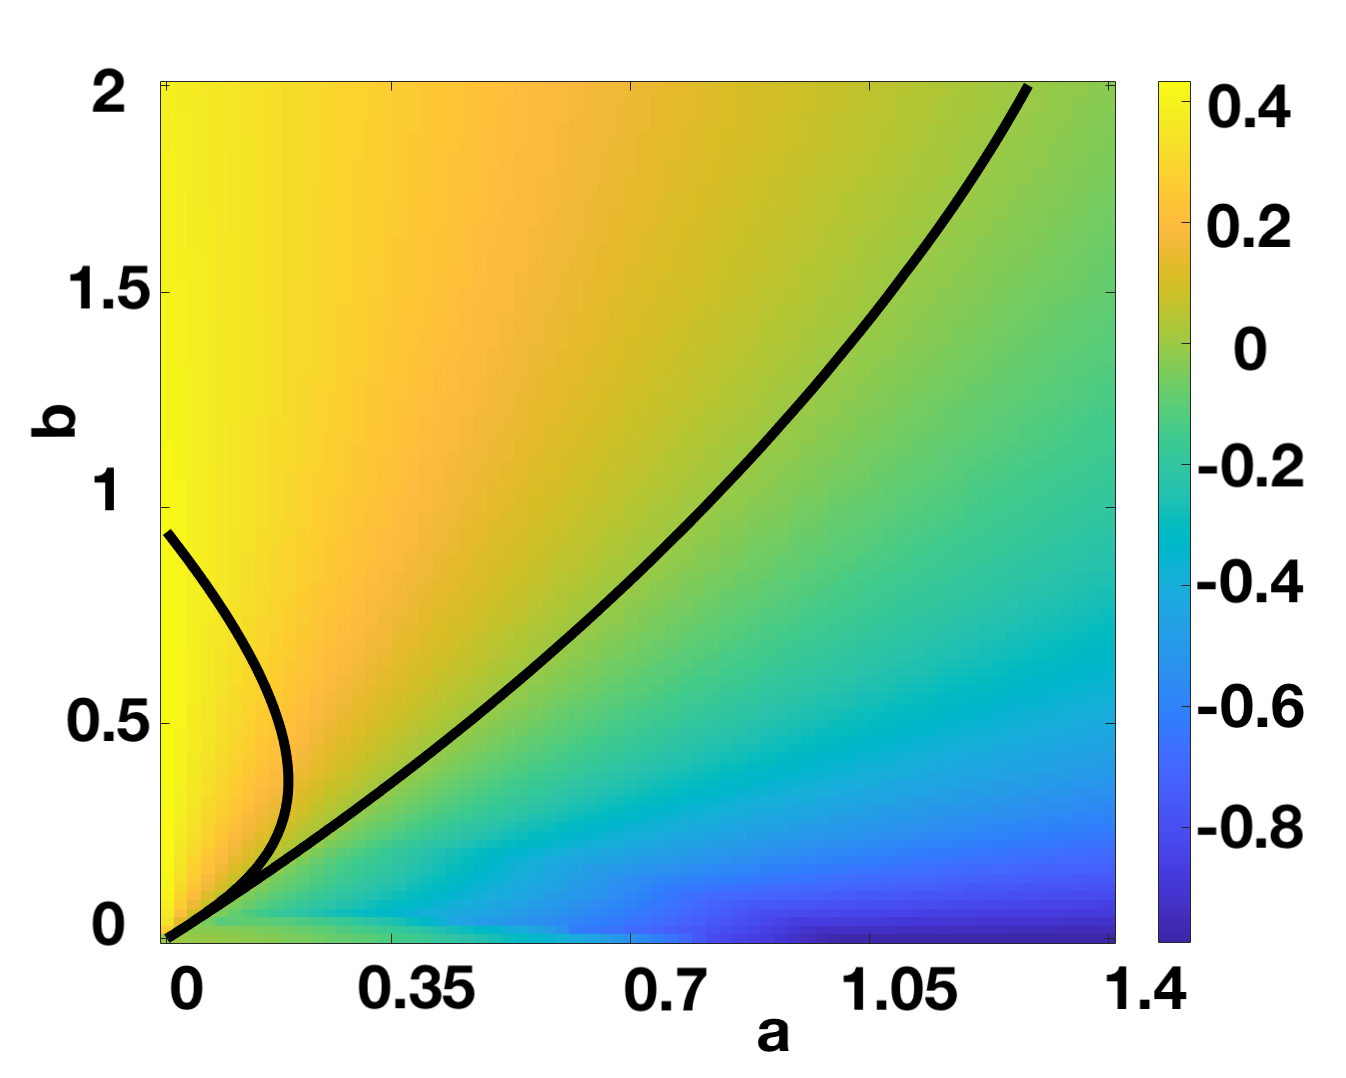
\includegraphics[width=7cm,height=4.75cm]{t1f4.png}
        \caption{Distributed delay with $\sigma=\sigma_{max}\times0.1$.}
        \label{}
    \end{subfigure}
    \caption{Bifurcation diagrams produced for $\tau=0.2$ and $\sigma=\{ \sigma_{max}\times0.99,\sigma_{max}\times0.2,\sigma_{max}\times0.1 \}$, compared with fixed delay case. $\epsilon^2=0.001$. }
    \label{fig:distbif1}
\end{figure}
\begin{figure}[H]
    \centering
    \begin{subfigure}[b]{0.45\textwidth}
        \centering
        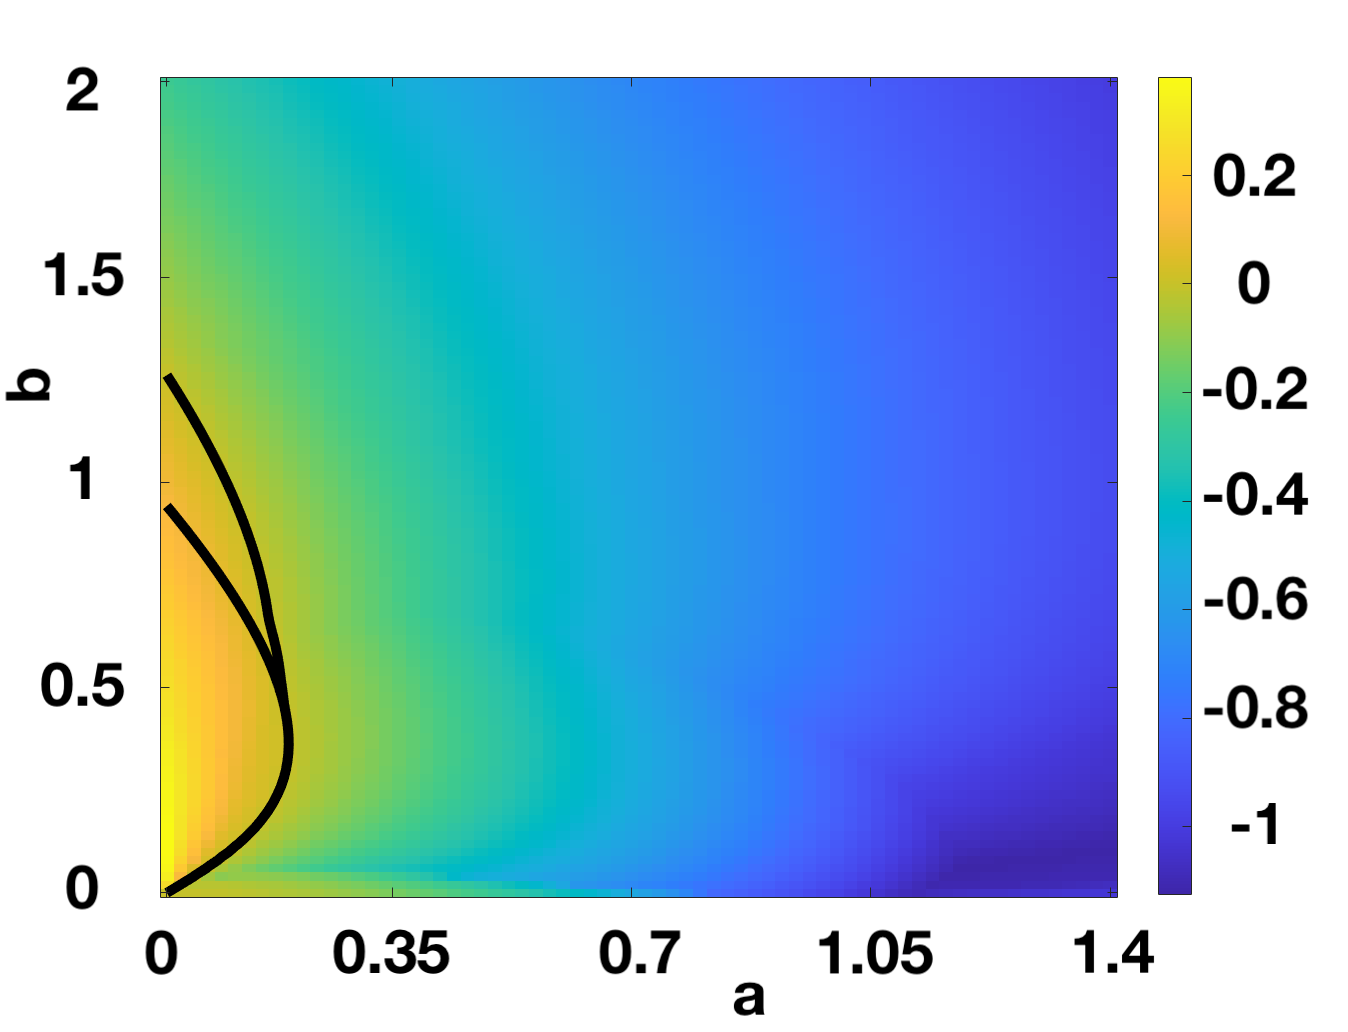
\includegraphics[width=7cm,height=4.75cm]{distbif31.png}
        \caption{Fixed delay case.}
        \label{}
    \end{subfigure}
    \hfill
    \begin{subfigure}[b]{0.45\textwidth}
        \centering
        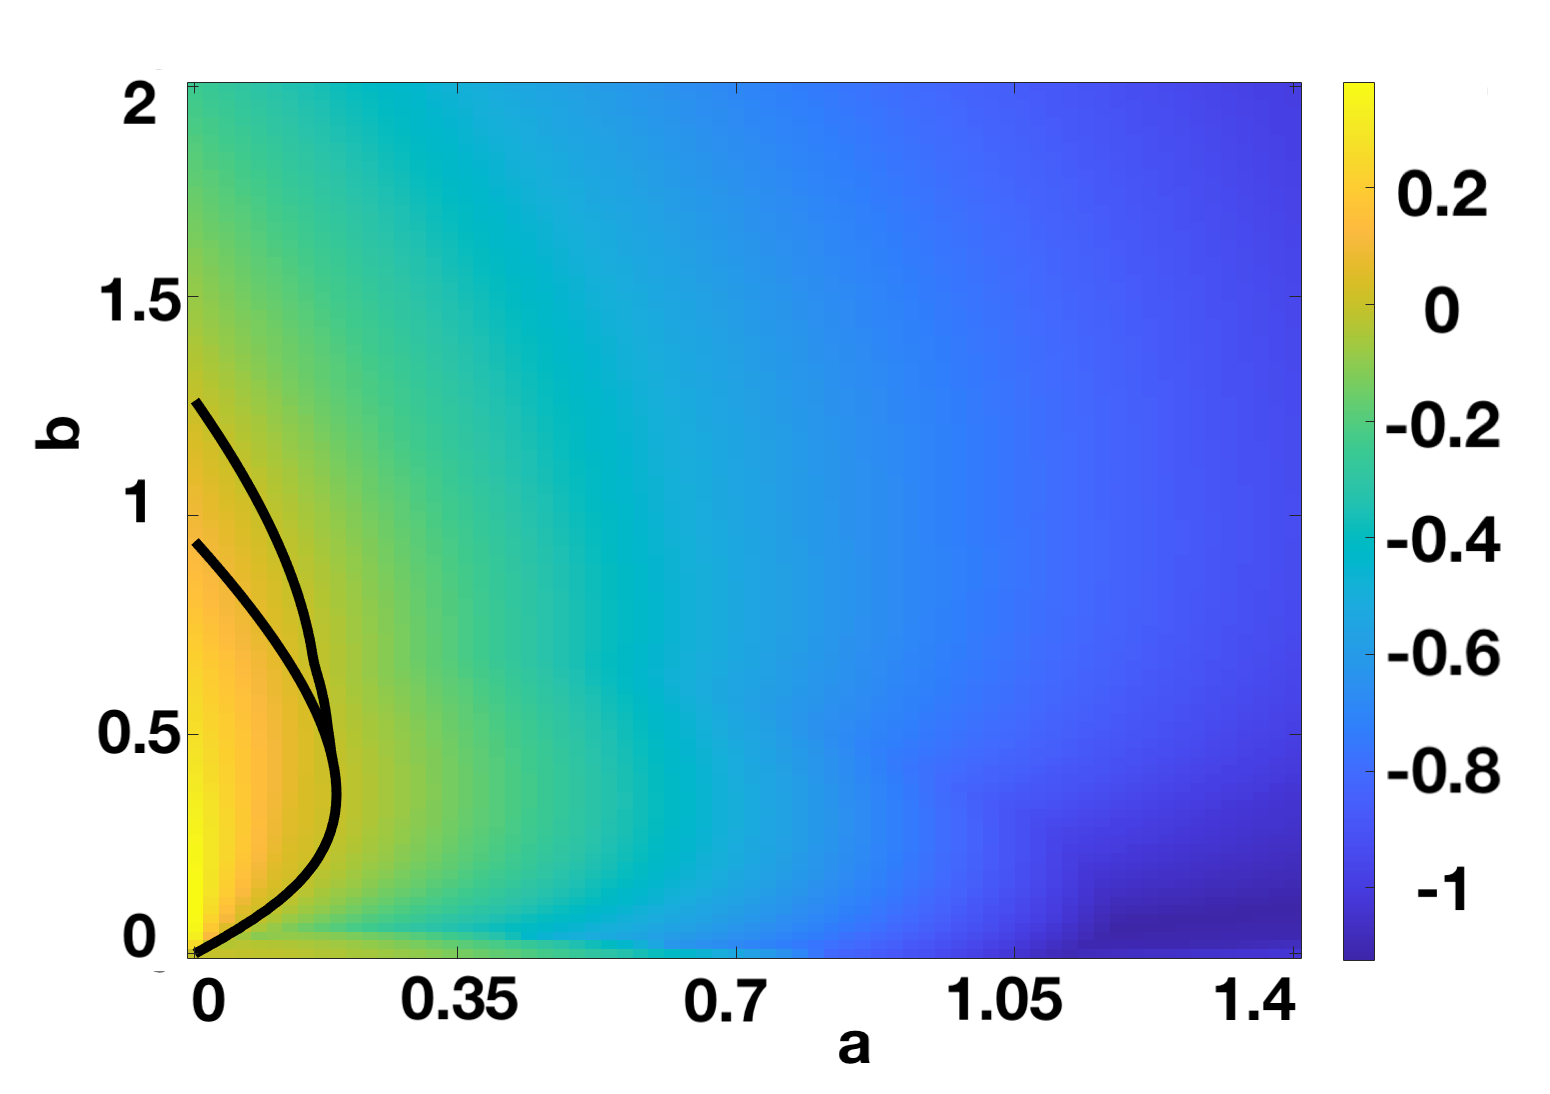
\includegraphics[width=7cm,height=4.75cm]{distbif32.png}
        \caption{Distributed delay with $\sigma=\sigma_{max}\times0.99$.}
        \label{}
    \end{subfigure}
    \hfill
    \begin{subfigure}[b]{0.45\textwidth}
        \centering
        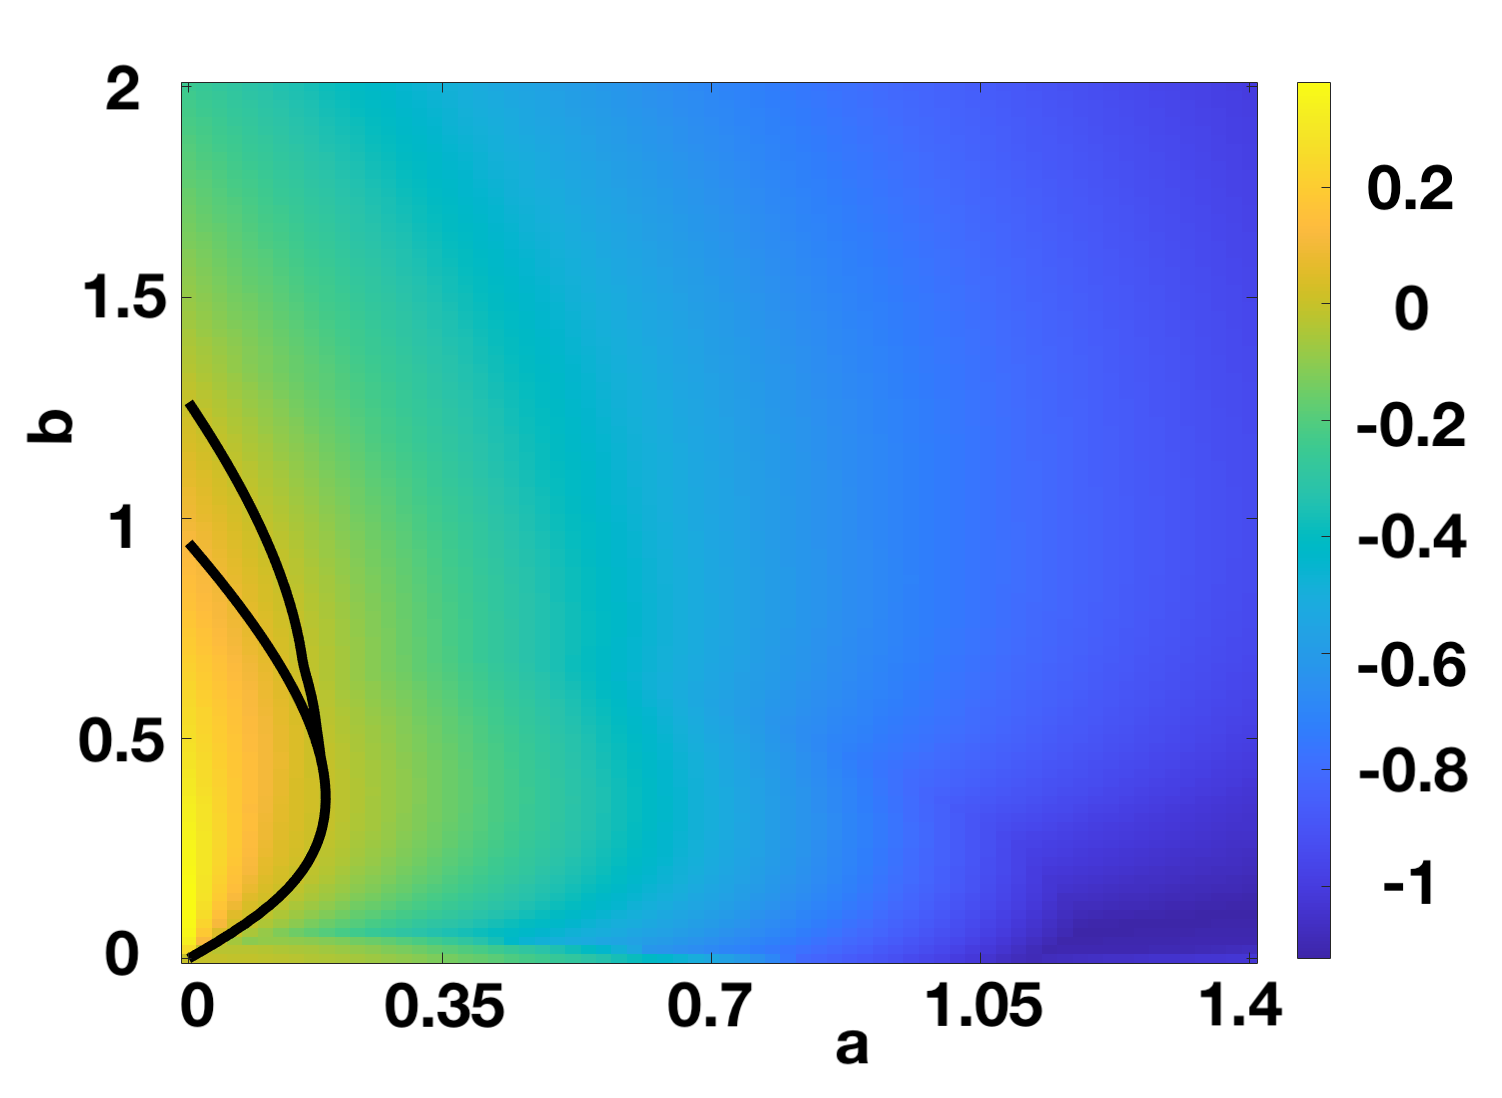
\includegraphics[width=7cm,height=4.75cm]{distbif33.png}
        \caption{Distributed delay with $\sigma=\sigma_{max}\times0.2$.}
        \label{}
    \end{subfigure}
    \hfill
    \begin{subfigure}[b]{0.45\textwidth}
        \centering
        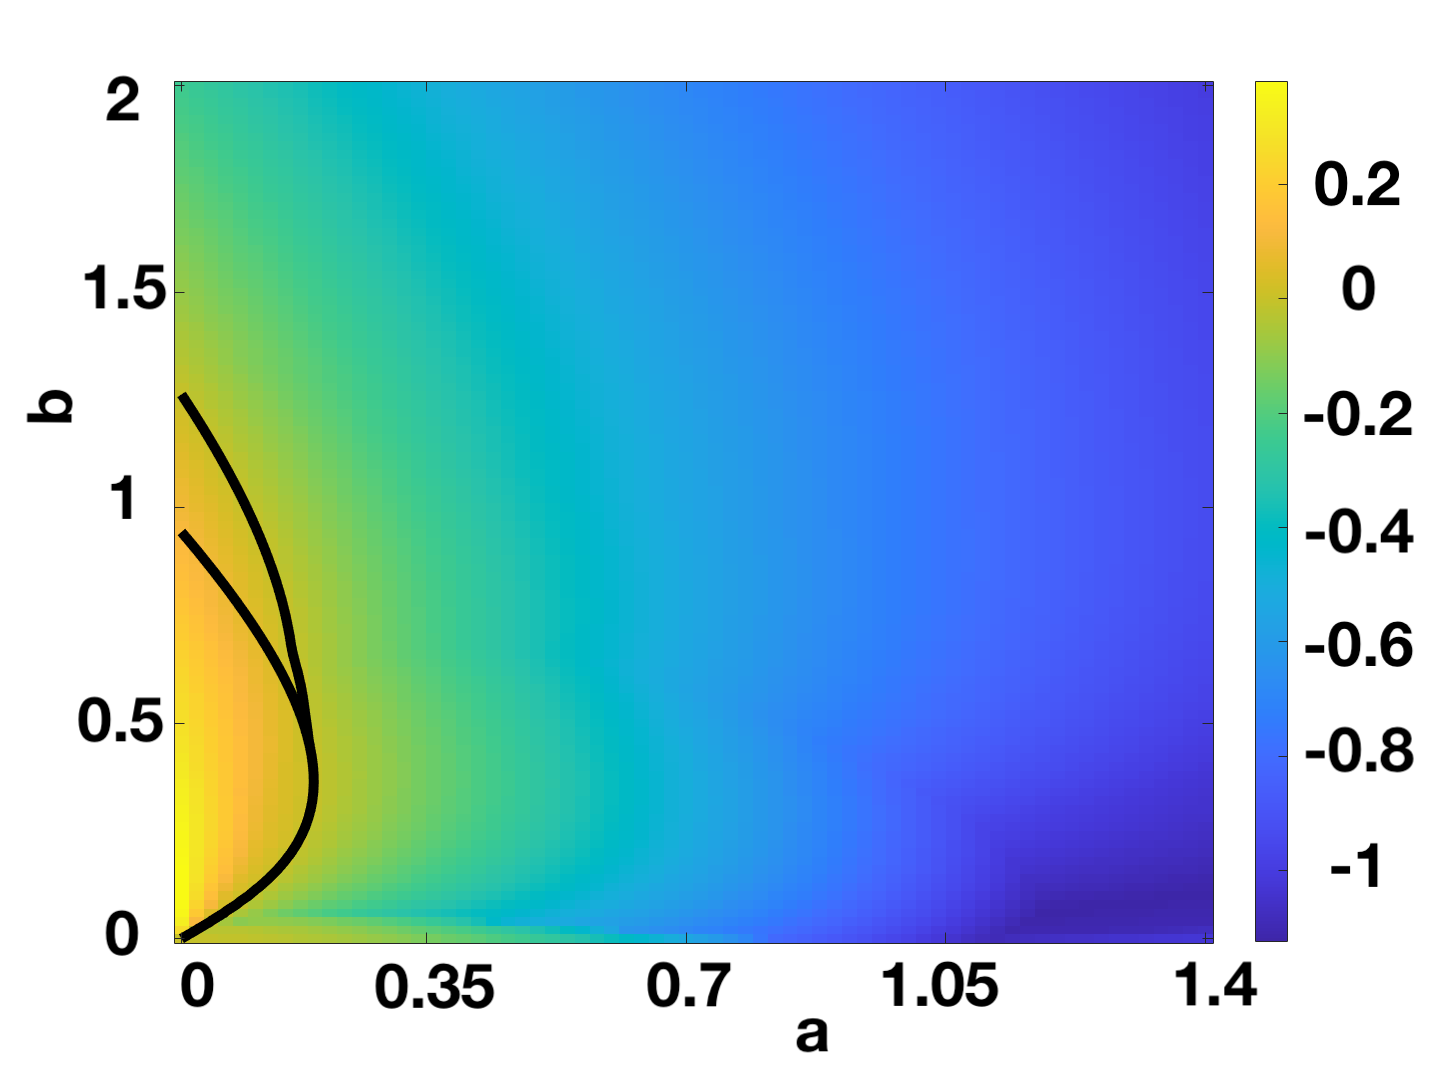
\includegraphics[width=7cm,height=4.75cm]{distbif34.png}
        \caption{Distributed delay with $\sigma=\sigma_{max}\times0.1$.}
        \label{}
    \end{subfigure}
    \caption{Bifurcation diagrams produced for $\tau=0.2$ and $\sigma=\{ \sigma_{max}\times0.99,\sigma_{max}\times0.2,\sigma_{max}\times0.1 \}$, compared with fixed delay case. $\epsilon^2=0.1$.}
    \label{fig:distbif3}
\end{figure}
\begin{figure}[H]
    \centering
    \begin{subfigure}[b]{0.45\textwidth}
        \centering
        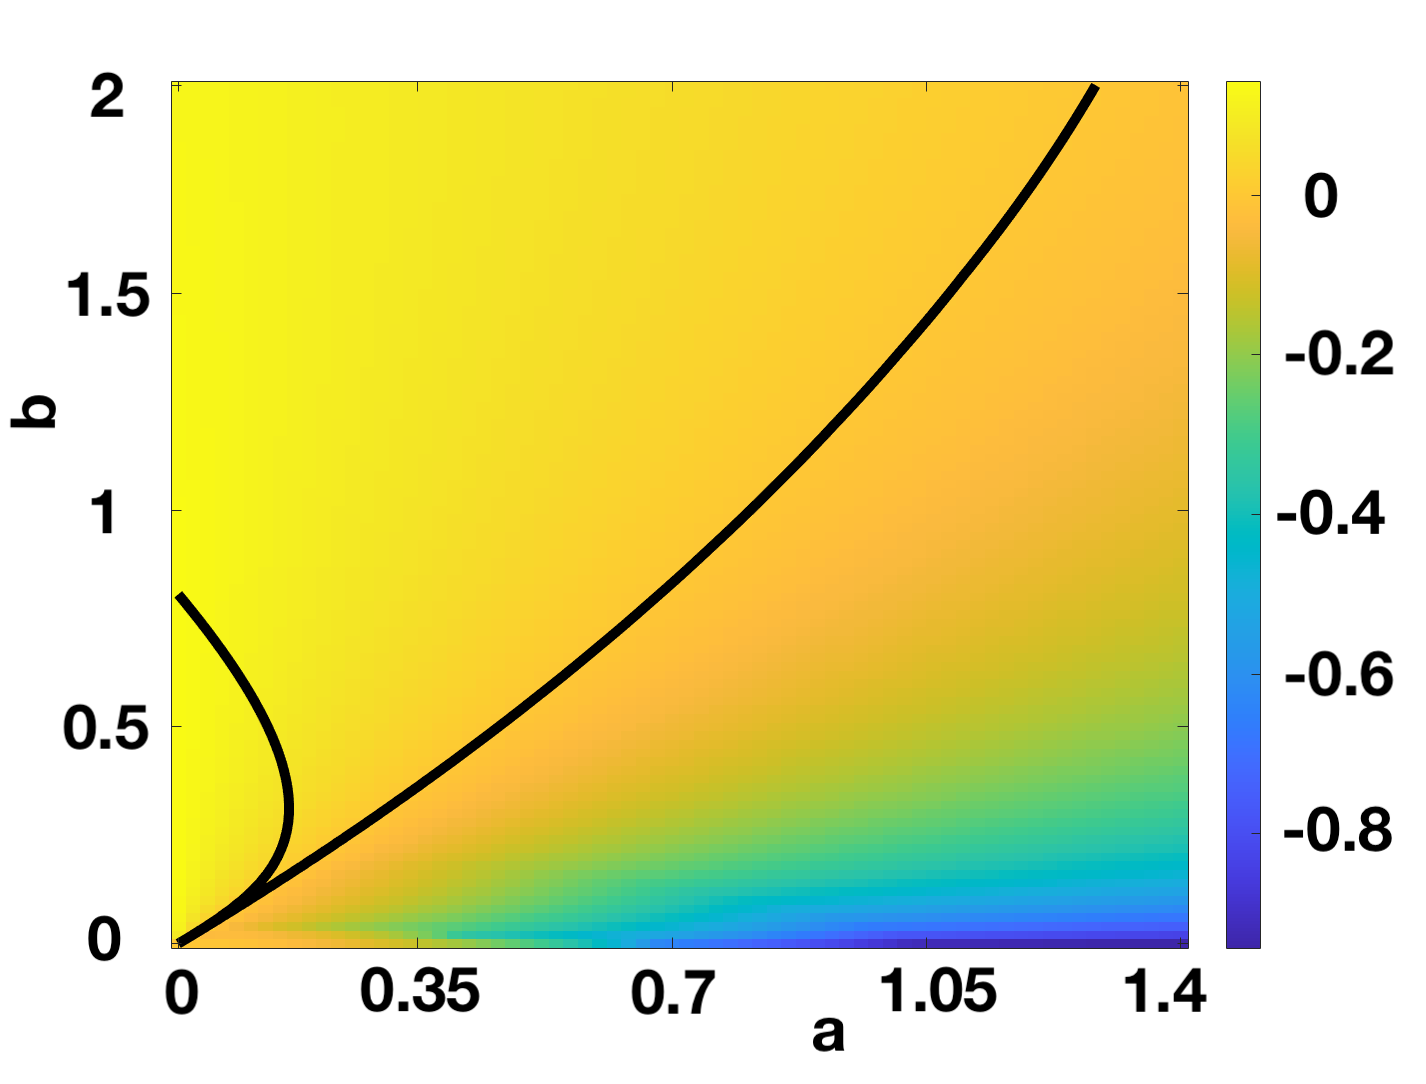
\includegraphics[width=7cm,height=4.75cm]{t2f1.png}
        \caption{Fixed delay case.}
        \label{}
    \end{subfigure}
    \hfill
    \begin{subfigure}[b]{0.45\textwidth}
        \centering
        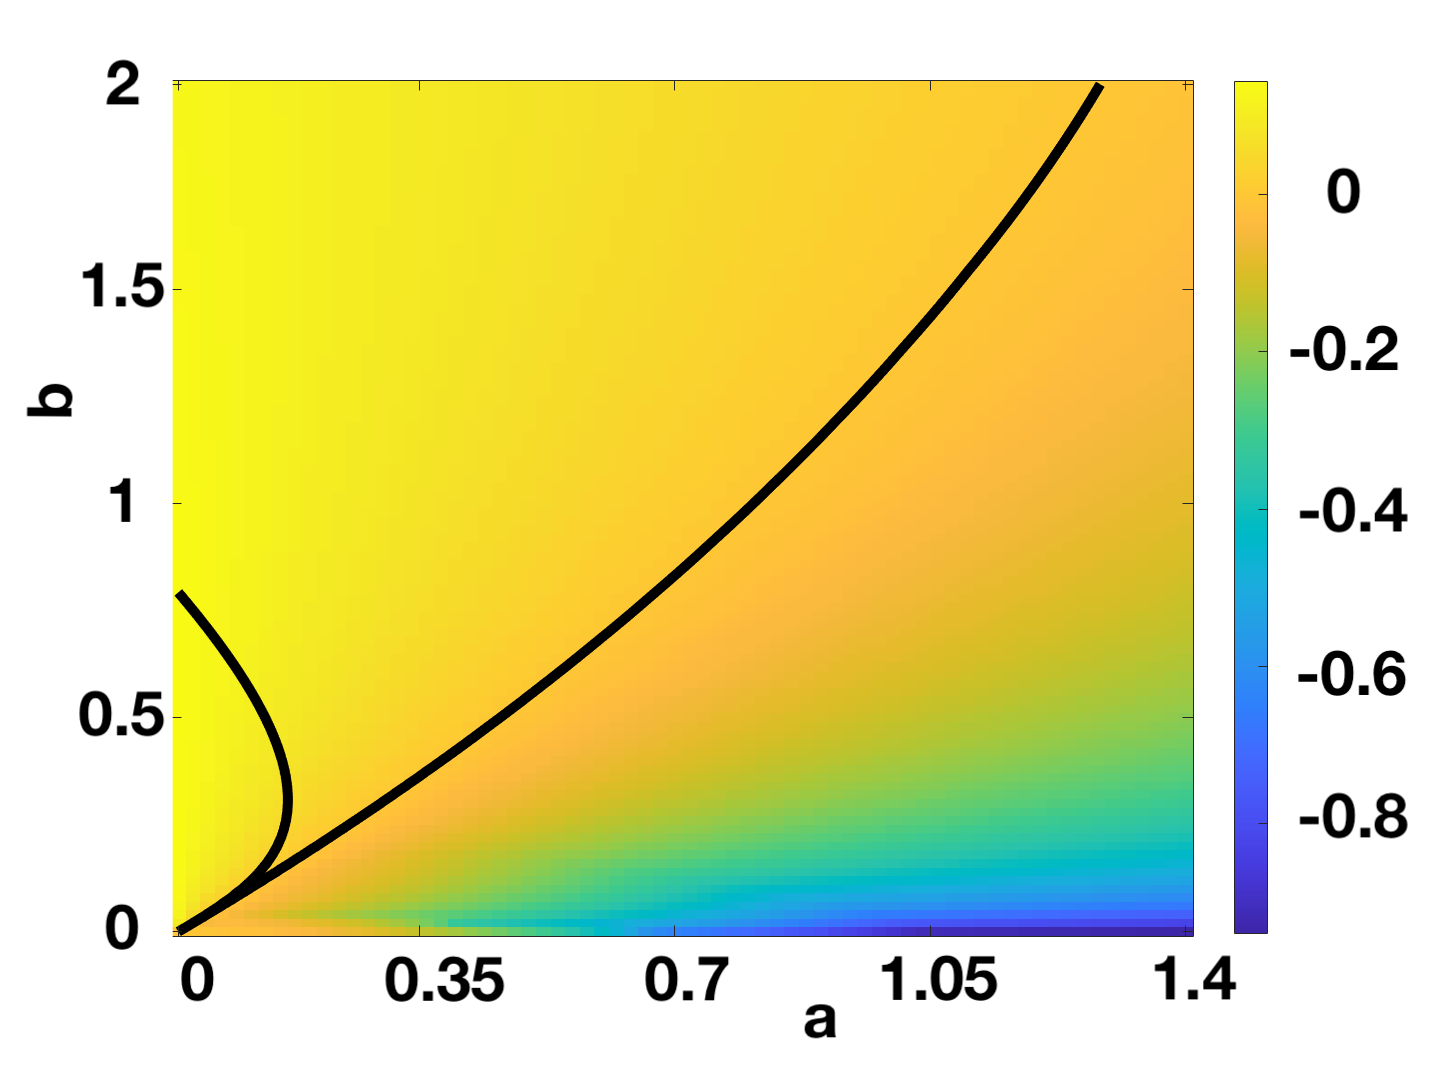
\includegraphics[width=7cm,height=4.75cm]{t2f2.png}
        \caption{Distributed delay with $\sigma=\sigma_{max}\times0.99$.}
        \label{}
    \end{subfigure}
    \hfill
    \begin{subfigure}[b]{0.45\textwidth}
        \centering
        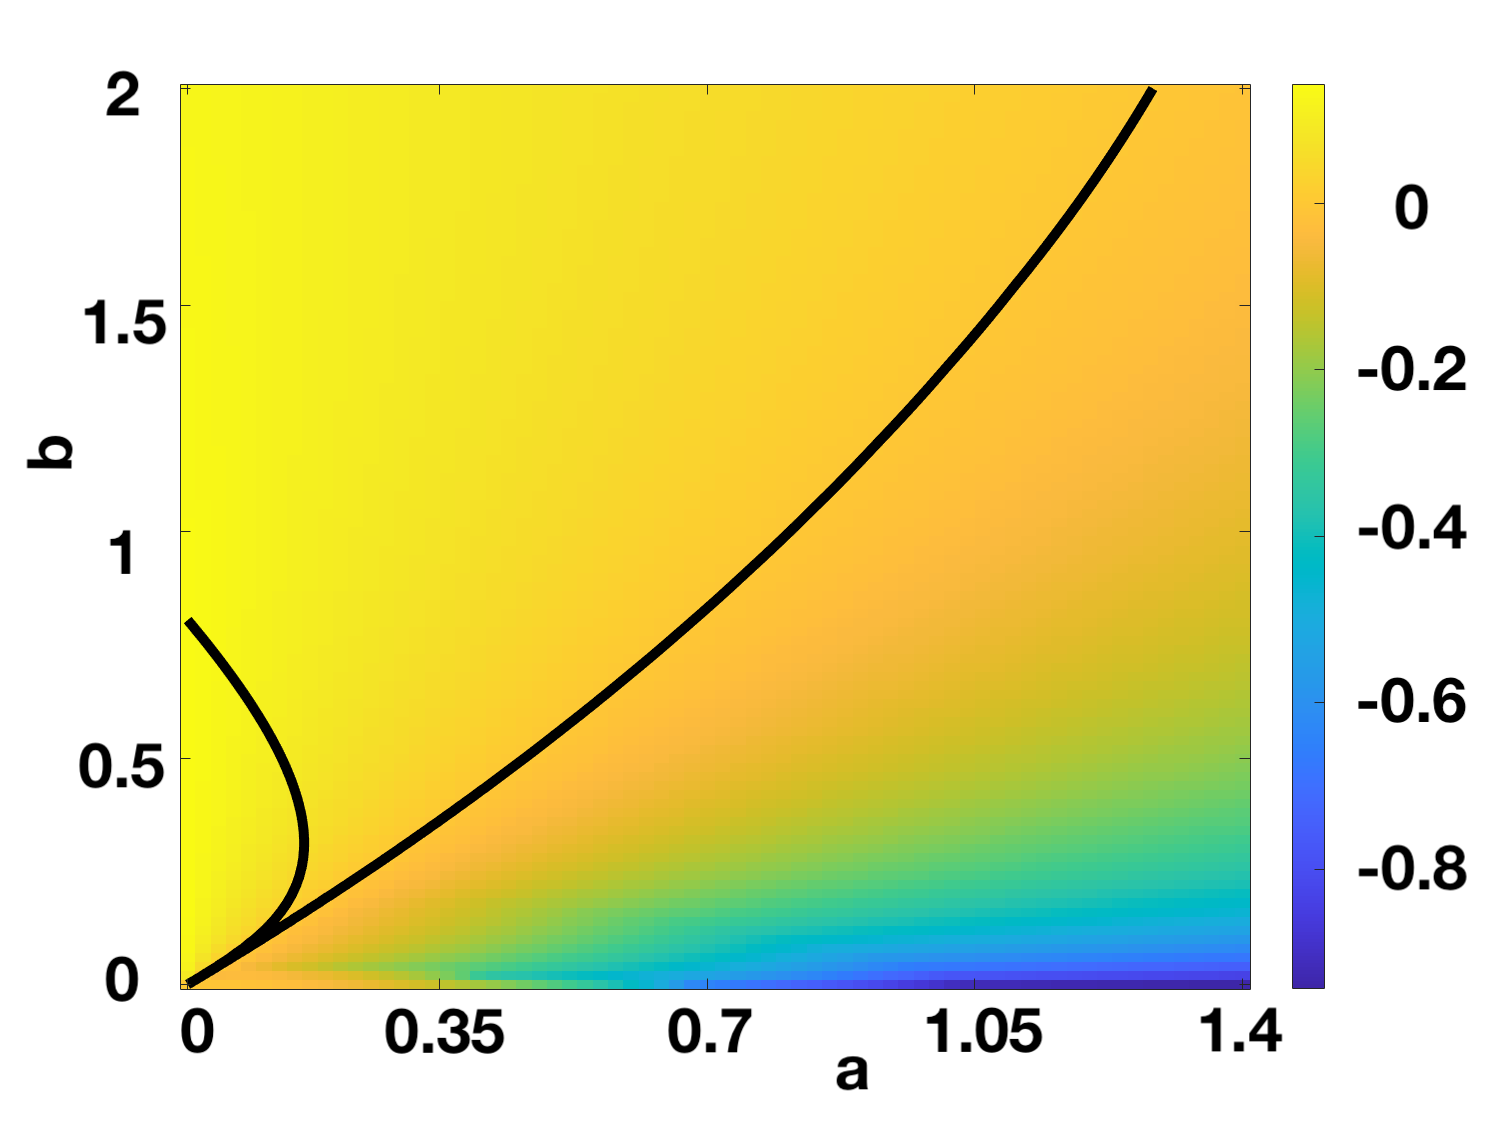
\includegraphics[width=7cm,height=4.75cm]{t2f3.png}
        \caption{Distributed delay with $\sigma=\sigma_{max}\times0.2$.}
        \label{}
    \end{subfigure}
    \hfill
    \begin{subfigure}[b]{0.45\textwidth}
        \centering
        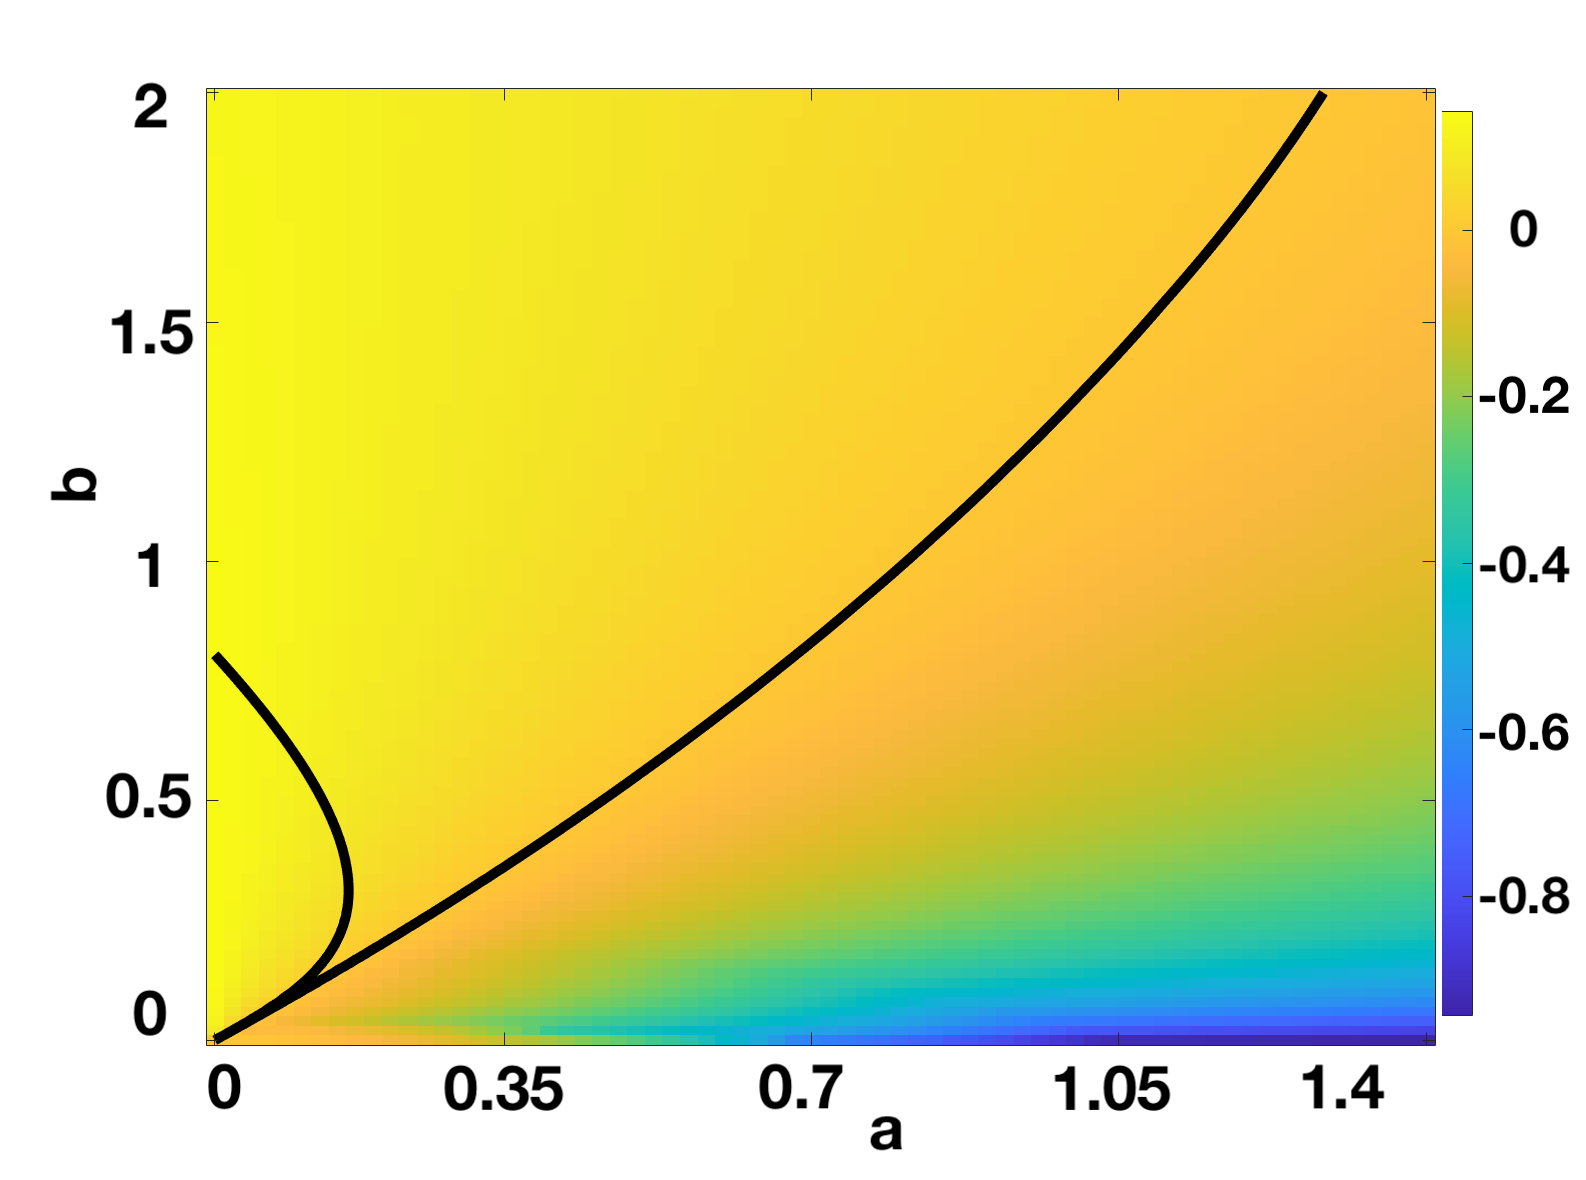
\includegraphics[width=7cm,height=4.75cm]{t2f4.png}
        \caption{Distributed delay with $\sigma=\sigma_{max}\times0.1$.}
        \label{}
    \end{subfigure}
    \caption{Bifurcation diagrams produced for $\tau=1$ and $\sigma=\{ \sigma_{max}\times0.99,\sigma_{max}\times0.2,\sigma_{max}\times0.1 \}$, compared with fixed delay case. $\epsilon^2=0.001$.}
    \label{fig:distbif2}
\end{figure}
\begin{figure}[H]
    \centering
    \begin{subfigure}[b]{0.45\textwidth}
        \centering
        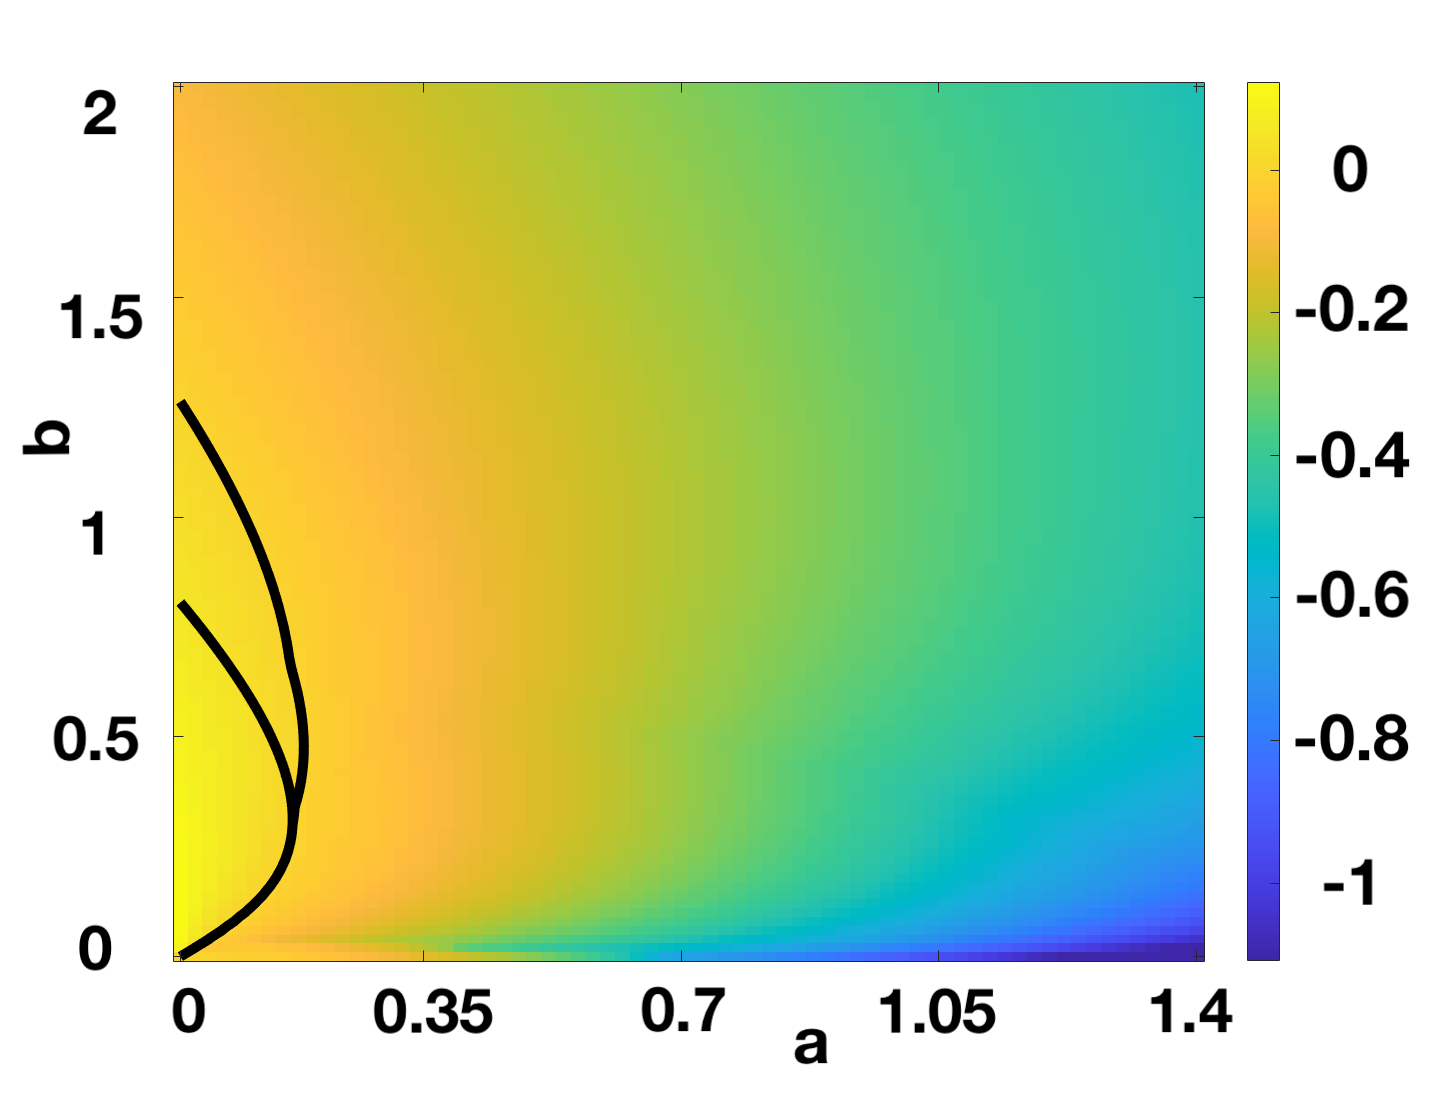
\includegraphics[width=7cm,height=4.75cm]{distbif41.png}
        \caption{Fixed delay case.}
        \label{}
    \end{subfigure}
    \hfill
    \begin{subfigure}[b]{0.45\textwidth}
        \centering
        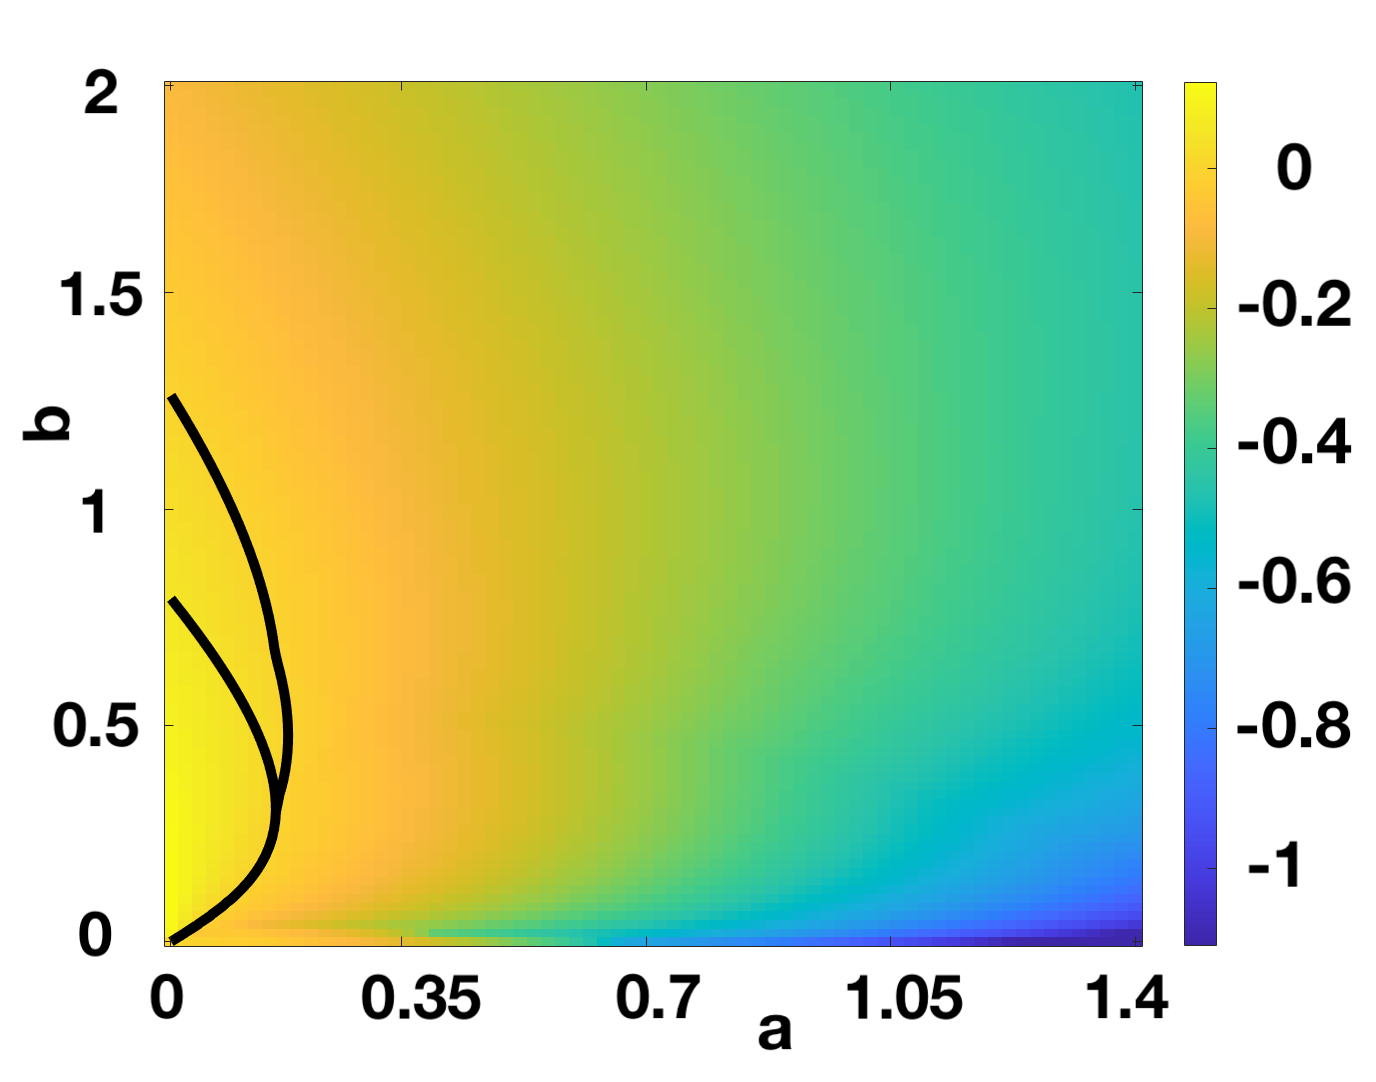
\includegraphics[width=7cm,height=4.75cm]{distbif42.png}
        \caption{Distributed delay with $\sigma=\sigma_{max}\times0.99$.}
        \label{}
    \end{subfigure}
    \hfill
    \begin{subfigure}[b]{0.45\textwidth}
        \centering
        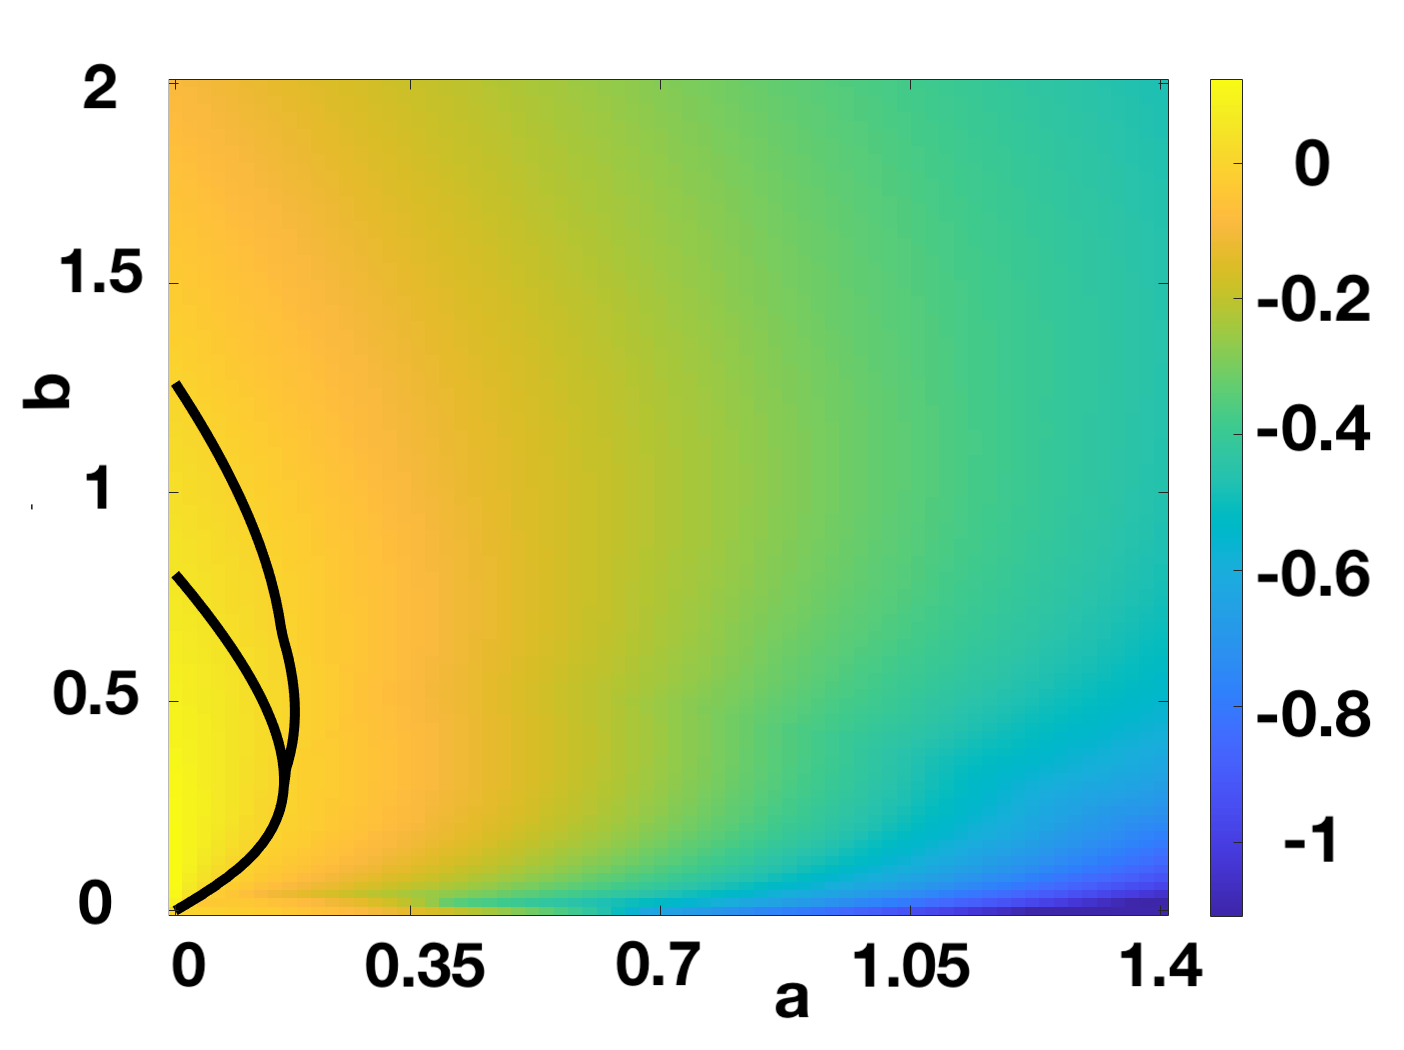
\includegraphics[width=7cm,height=4.75cm]{distbif43.png}
        \caption{Distributed delay with $\sigma=\sigma_{max}\times0.2$.}
        \label{}
    \end{subfigure}
    \hfill
    \begin{subfigure}[b]{0.45\textwidth}
        \centering
        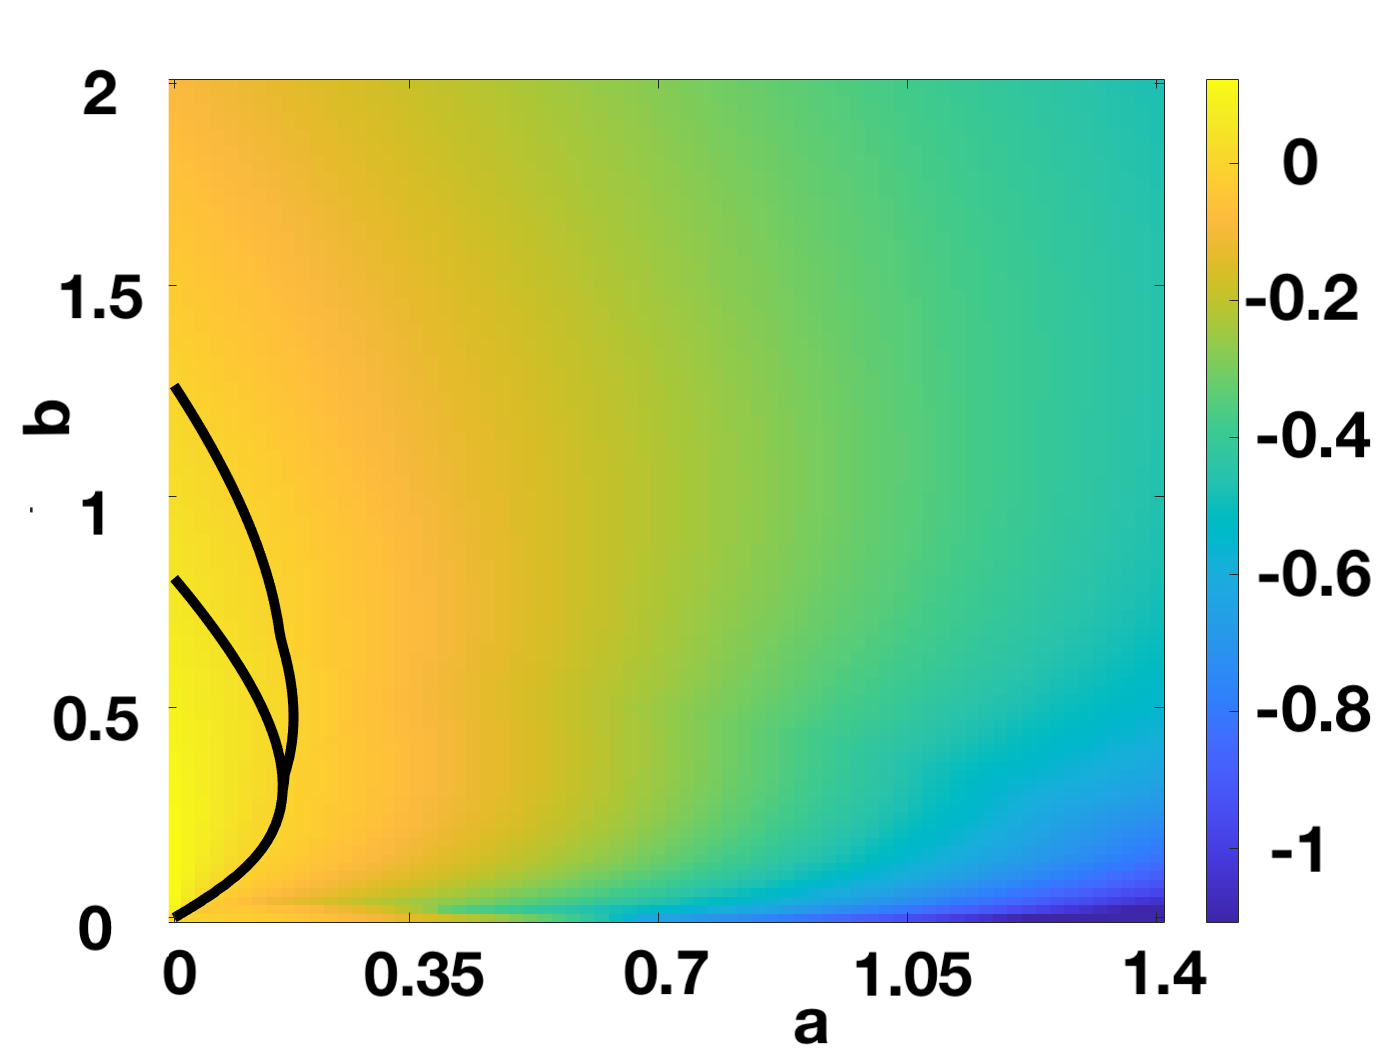
\includegraphics[width=7cm,height=4.75cm]{distbif44.png}
        \caption{Distributed delay with $\sigma=\sigma_{max}\times0.1$.}
        \label{}
    \end{subfigure}
    \caption{Bifurcation diagrams produced for $\tau=1$ and $\sigma=\{ \sigma_{max}\times0.99,\sigma_{max}\times0.2,\sigma_{max}\times0.1 \}$, compared with fixed delay case. $\epsilon^2=0.1$.}
    \label{fig:distbif4}
\end{figure}

We see that, for $\tau=0.2$, $|\max_k(\Re(\lambda_k))|$ is larger than that of $\tau=1$ for both $\epsilon^2$ values and all $\sigma$ values plotted. We also observe that the bifurcation diagrams do not change as $\sigma$ is varied, independent of the diffusion ration used. We therefore expect that for all $(a,b)\in[0,1.4]\times[0,2]$, using a symmetric Gaussian distribution centred at some mean $\tau$ will not effect the time-taken until pattern formation for a fixed delay of $\tau$, irrespective of the standard deviation $\sigma$ of the distribution.


\section{Numerical Results}\label{section:distsim}
Numerical simulations are presented here to confirm the linear theory presented in section \ref{section:distlin}. Through numerical simulation, for various parameter sets $(a,b,\tau,\sigma,\epsilon^2)$, we show that the time taken until pattern formation does not change as $\sigma$ varies for a fixed $(a,b,\tau,\epsilon^2)$, compared to that of the fixed delay case with a time-delay $\tau$.
